\section{Measurement of the \SD telescope response}
\label{sec:rsd}
\label{sec:sd_datadesc}

In this section, we present the measurement of the \SD telescope response $\Rtel(\lambda)$ from CBP shoots using the \spinhole pinhole. One difficulty is the intercalibration between the \spinhole pinhole and the \bpinhole pinhole with which the CBP transmission has been determined in the previous section. Both produce images that are contained in the \SD sensor as shown in Figure~\ref{fig:ccd_examples}, but the latter form an image of about 250 pixels in radius while the first forms an image of about 4 pixels in radius. Their photometry is thus very differently affected by issues such as ghost reflection and light scattered in the tails of the PSF. In this section we start by building a model of the PSF of \SD+CBP  including the reflection of light in the optics. We use this model to correct the intercalibration ratio between the two pinhole sizes, measured with run No.~8 data. We then describe the generic photometry method applied to all other runs using the \spinhole pinhole data, and present the resulting response measurements.   

\begin{figure}[h]
    \centering
    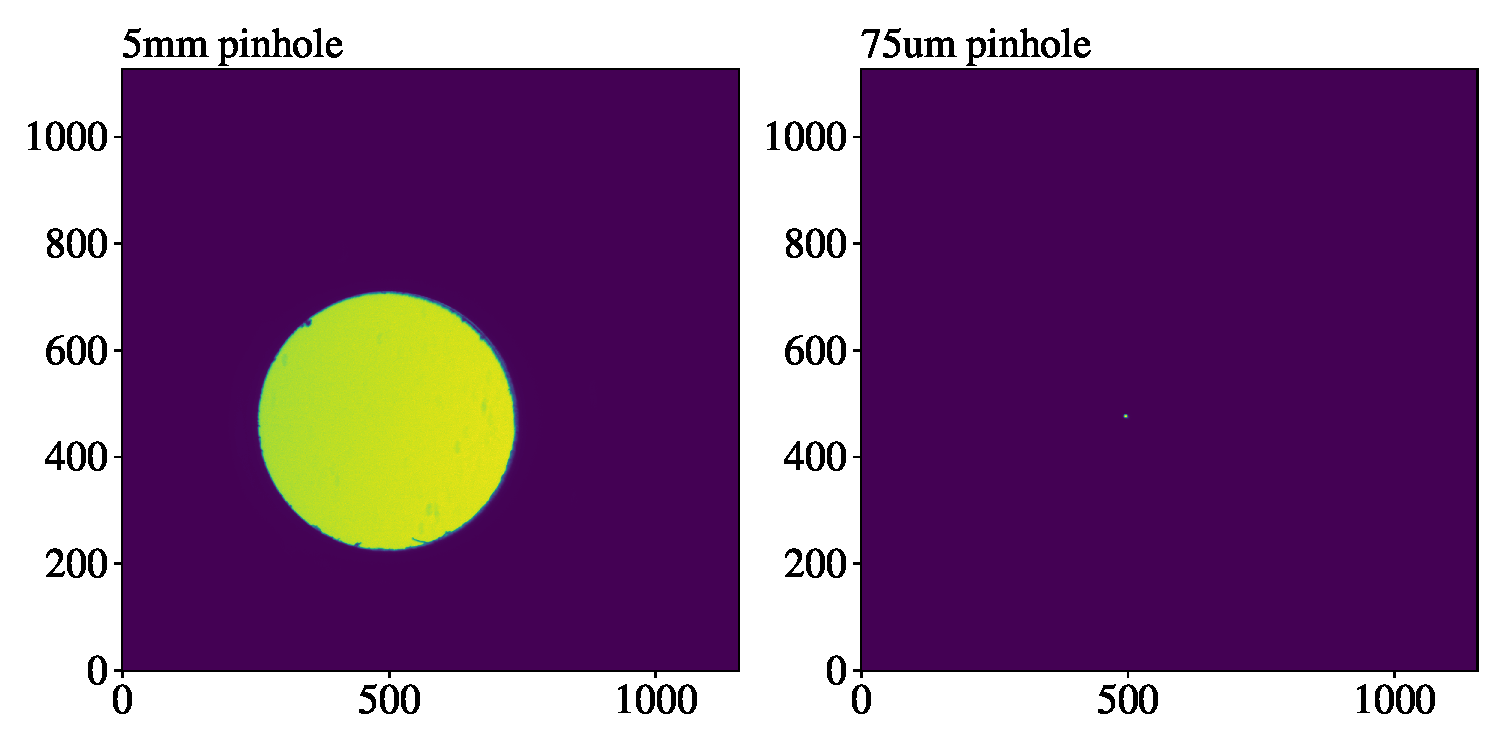
\includegraphics[width=\columnwidth]{fig/ccd_examples.pdf}
    \caption{Examples of images obtained when the CBP shoots in the \SD telescope at $\lambda_L=\SI{450}{\nm}$ with the \bpinhole pinhole on the right and \spinhole pinhole on the left. The ghost reflection is visible for both images at the left of the main spot. In the \bpinhole pinhole image, a large annulus around the main spot is visible and corresponds to light diffusion around a mechanical iris at the input of the CBP.}
    \label{fig:ccd_examples}
    %~/stardice/analysis/cbp_paper/total_fluxes/ghost_stack_figure.ipynb
\end{figure}


\subsection{Modelisation of the \SD PSF on \spinhole pinhole data}
\label{sec:modelisation-sd-psf}

Figure~\ref{fig:ghost_contrast} shows stacks of images obtained with the \spinhole pinhole in the absence of any filter. The illumination of a section of the primary StarDICE mirror results in a superimposition of the \SD telescope PSF, and a set of additional fainter images that we call ghosts. The ghosts result from undesired but unavoidable reflections on optical surfaces. The most visible ones come from the beam reflection on the CCD surface and back reflection on its covering window, as described in Figure~\ref{fig:schema_ghost}.\\

\begin{figure}[h]
    \centering
    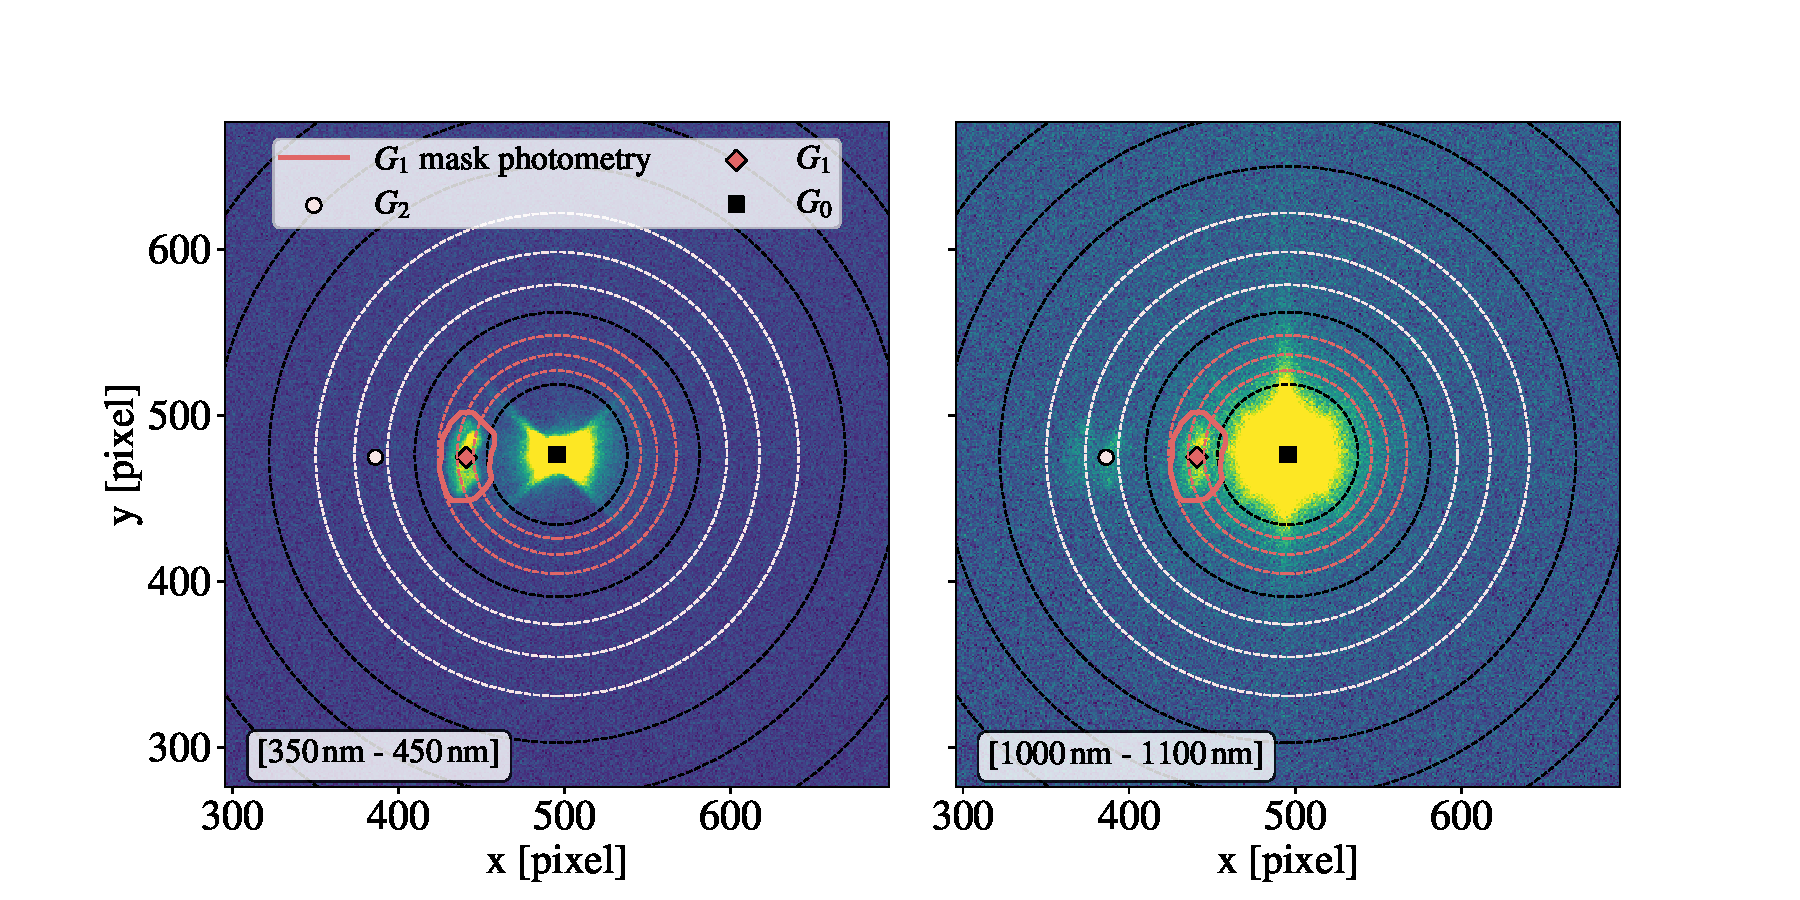
\includegraphics[width=\columnwidth]{fig/ghost_contrast.pdf}
    \caption{Stack of images at different wavelengths, with one image per nanometer. \textit{Left:} Stack of images between \SI{350}{\nano\meter} and \SI{450}{\nano\meter}. The scale is set on the ZScale from IRAF to make faint features visible. The spot of interest $G_0$ is at the center, and the ghost reflections are at its left. The circles correspond to the aperture photometry at different radii, when an annulus contains ghost contribution, it is colored with respect to the order of the ghost. The red area around the 1$\up{st}$ order ghost represents the area where the photometry of the ghost is measured. \textit{Right:} Same image but for a stack of images between \SI{1000}{\nano\meter} and \SI{1100}{\nano\meter}. We note that the 2$\up{nd}$ order ghost is not visible for the stack in the UV, where the 1$\up{st}$ order is maximal, while it is visible in the IR, where the 1$\up{st}$ order is lower.}
    \label{fig:ghost_contrast}
    %~/stardice/analysis/cbp_paper/total_fluxes/ghost_stack_figure.ipynb
\end{figure}

For each image in this dataset, we subtract a bias pattern, estimated on a column and row basis by computing the mean of the horizontal and vertical overscans. We then perform aperture photometry by summing pixels within a radius $r=\SI{20.9}{pixels}$, and then for successive annulus of external radius from \SI{24.9}{pixels} to \SI{419.1}{pixels}. These radii are regularly spaced on a logarithm scale shown in Figure~\ref{fig:ghost_contrast}.

%The overscan estimates are obtained as the mean n of each column $i$ of the horizontal overscan and each row $j$ of the vertical overscan is computed. For each pixel $(i, j)$, we subtract the sum of the estimation of the overscan estimated on the column $i$ and the row $j$. \\
We model the \SD telescope PSF as the sum of a Moffat function, a constant background level, and contributions from ghosts at specific distances from the main spot. The Moffat function \citep{moffat}, integrated in an aperture of radius $r,$ writes:
\begin{equation}
M(r, \lambda)= 1 - \left( 1+\frac{r^2}{\alpha(\lambda)^2} \right)^{1-\beta(\lambda)},
\end{equation}
with $\alpha(\lambda)$ and $\beta(\lambda)$ the scale and exponent parameters of the Moffat distribution which depend on the wavelength. The flux $F(r, \lambda)$ measured in the CCD with aperture photometry, can then be modeled as: 
\begin{equation}
F(r, \lambda) = A(\lambda) \times \frac{M(r, \lambda) + \Kghostfit(r, \lambda)}{1 + \Kghostfit(r \rightarrow +\infty, \lambda)} + \pi r^2 bkg(\lambda),
\label{eq:moffat_model}
\end{equation}
with $A(\lambda)$ the total amplitude, $\Kghostfit(r, \lambda) = \frac{\sum_{n=1}^{+\infty} G_n(\lambda)}{A(\lambda)}$ the relative contribution of the sum of all the ghosts $G_n(\lambda)$, and $bkg(\lambda)$ the background level in ADU/pixel. 

The evolution of the Moffat distribution is smooth with respect to wavelength. We therefore develop the parameters $\alpha(\lambda)$ and $\beta(\lambda)$  on a B-spline basis with 15 wavelength nodes regularly spaced between \SI{350}{\nano\meter} and \SI{1100}{\nano\meter}. The same applies to the function $\Kghostfit(r, \lambda)$ as it corresponds to light reflections on surfaces in the optical path. This reduces the number of free parameters and allows us to perform outlier rejection of a few annulus whose photometry was affected by a cosmic ray (9 photometric points affected out of 13122 measurements). The results of the fit are shown in Figure~\ref{fig:result_params}. 

\begin{figure}[h]
    \centering
    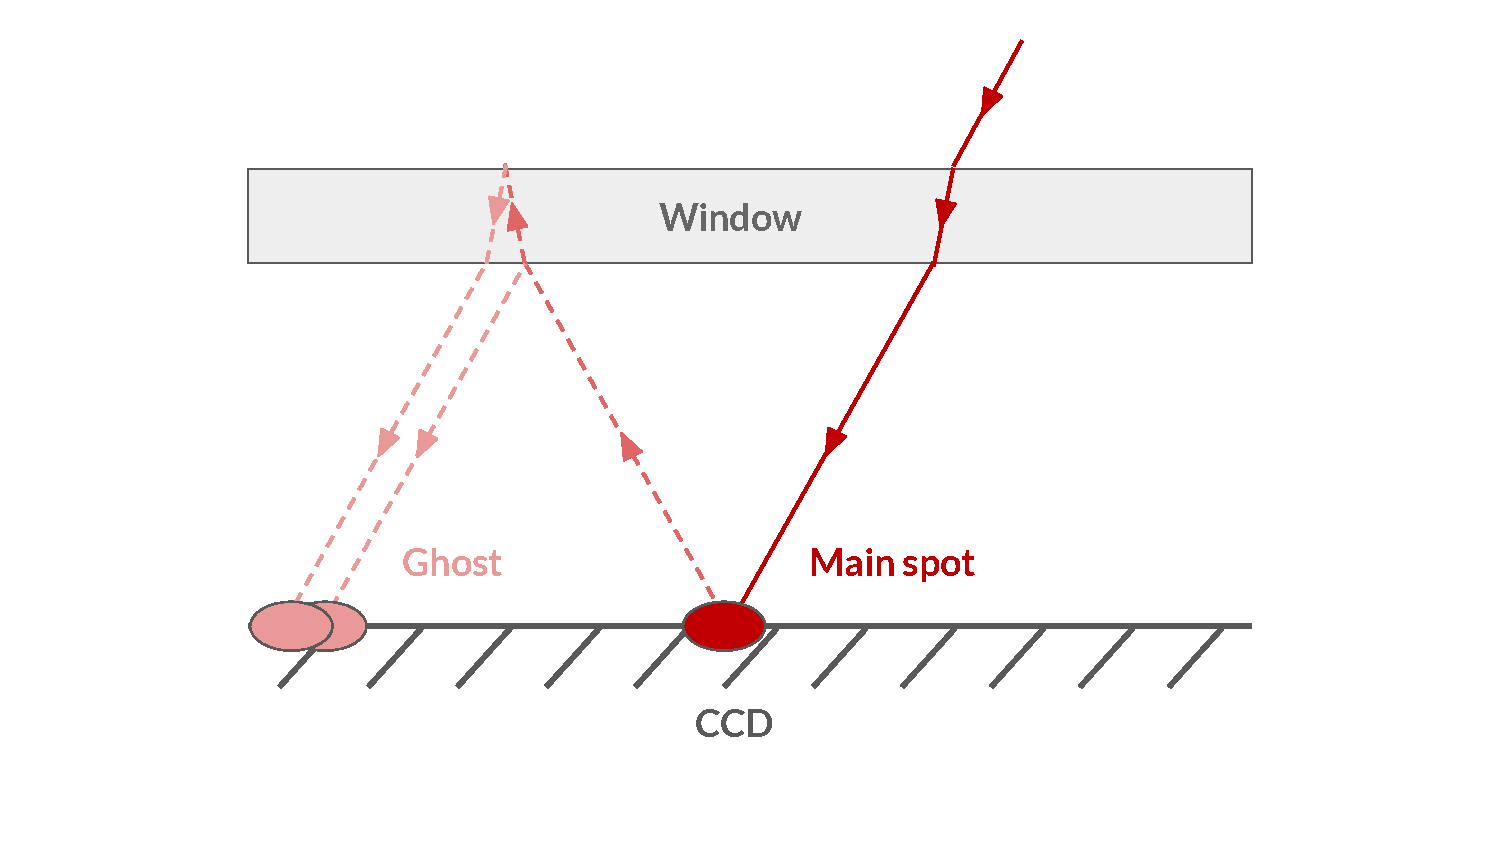
\includegraphics[width=\columnwidth]{fig/schema_ghost.pdf}
    \caption{Schematic of the light reflections that generate the ghosts, which are defocused and less intense images at other positions in the focal plane. A fraction of the light is reflected at the different interfaces and $G_0(\lambda)$, $G_1(\lambda)$ and $G_2(\lambda)$ are respectively the main spot, the 1\up{st} order ghost, and the 2\up{nd} order ghost.}
    \label{fig:schema_ghost}
    %Google slides
\end{figure}

The most striking result is a significant degradation of the PSF
after \SI{950}{nm}, apparent in the steep decrease of the value of
the $\beta$ Moffat parameter and the increase of the $\alpha$
parameter presented in the first and second panels. This effect is also
visible when comparing the two stacks in
Fig.~\ref{fig:ghost_contrast}. We were not able to pin down the exact
origin of this degradation. A potential explanation could be that one
of the reflective surfaces becomes partially transparent at these
wavelengths and generates diffused light. The consequence of this
effect on photometry will be further discussed in Section \ref{sec:photometry_small}.

The $\alpha(\lambda)$ and $\beta(\lambda)$ best-fit parameters are
otherwise fairly stable between \SI{350}{\nano\meter} and
\SI{900}{\nano\meter}. The third panel shows the background level
reconstructed across all wavelengths. With a mean of
$\mu_\mathrm{bkg, fitted}=\SI{0.267}{ADU/pixel}$ for an exposure time
of \SI{1.1}{\second}, it is very consistent with the values measured
on dark images. Two datasets of dark images have been studied, one
with the laser turned off, and a second by masking the CBP output with
a cap (dataset No.~9 in Table~\ref{tab:schedule}). Both datasets show
no trend in time or wavelength and have a mean value of
$\mu_\mathrm{dark, photometry}=\SI{0.252}{ADU/pixel}$ and a standard
deviation $\sigma_\mathrm{dark, photometry}=\SI{0.059}{ADU/pixel}$,
represented by the black dashed line and shaded area in this third
panel.

The fourth panel presents the relative contribution of the first order
ghost $G_1(\lambda)$,
$\Kghostfitfirst(\lambda) = \frac{G_1(\lambda)}{A(\lambda)}$ in
percent. We compared these reconstructed values with direct photometry
of the visible first order ghost pattern performed in 2D images as
detailed in Appendix~\ref{sec:ghost_photometry}. This more direct
determination of the ratio $\Kghost$ is shown as the dashed black
line. The two different methods match perfectly up to \SI{950}{nm}
showing that the identified ghost constitutes the only significant
deviation from the Moffat profile. Beyond \SI{950}{nm} the second method
does not give an accurate photometry for the ghost because it starts
to be mixed with the core of the PSF.

%fraction $\Kghost=\frac{G_1(\lambda)}{G_0(\lambda)}$ obtained by photometry measurements on the first order ghost $G_1(\lambda)$ and the main spot $G_0(\lambda)$. The method to perform ghost photometry. The ratio and $\Kghostfitfirst$ obtained with two different methods on two different datasets are superimposing well below \SI{950}{\nano\meter}, which gives us confidence about the accuracy of this measurement. The deviation above \SI{950}{\nano\meter} between the two methods can be explained by the following arguments. the $\alpha(\lambda)$ and $\beta(\lambda)$ parameters indicate a deterioration of the PSF, which starts to overflow in the ghost photometry. In addition, interference fringes are appearing in the focal plane at these wavelengths, complicating the ghost photometry. As the fit accounts for the PSF evolution, the fitted result gives more confidence in its accuracy.

The fit reduced chi-squared of 1.86 is explained by the fact that the Moffat
shape does not describe the complex shape of the PSF core. To mitigate this
issue, and as we are mainly interested in modeling the tails of the PSF, we
start our profile modeling at a rather large inner aperture of 20.9 pixels where
residuals no longer display visible structure and the chi-square displays no
trend in wavelength. Going to a larger inner aperture increases the quality of
the fit but decrease its stability as the scale parameter $\alpha$ is no longer
properly constrained.

\begin{figure}[h]
     \centering
     \resizebox{\hsize}{!}{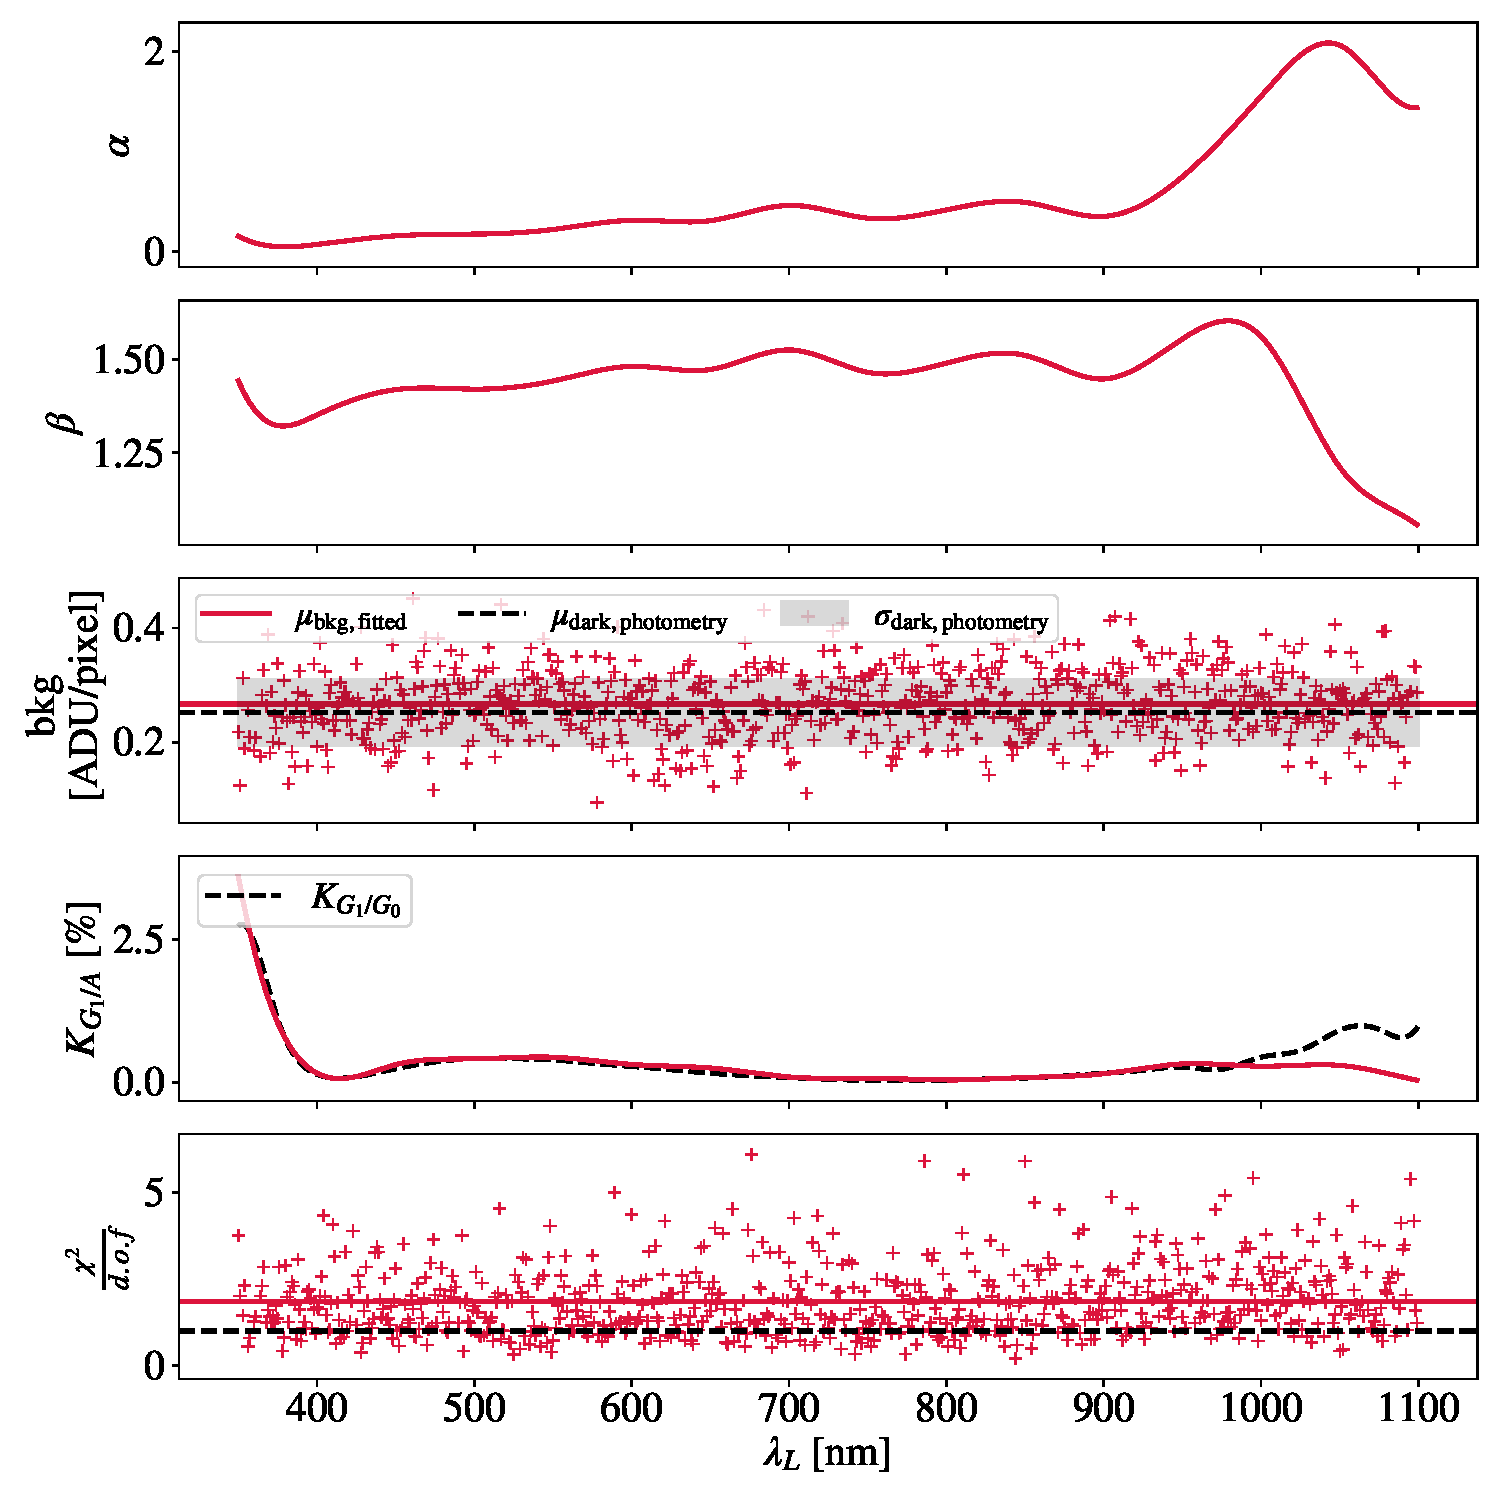
\includegraphics{fig/result_params.pdf}}
     \caption{Best fitting parameters for the model of Equation~\ref{eq:moffat_model}. Red plain lines correspond to the result of the fit, and black dashed lines, when applicable, correspond to the values expected. From top to bottom: the first and second panels represent respectively the $\alpha(\lambda)$ and $\beta(\lambda)$ parameters from the Moffat distribution; the third panel shows the background contribution per pixel and its mean value in red, while the dark dashed line is the mean value of the dark; the fourth panel represents $\Kghostfitfirst(\lambda)$, and $\Kghost$; the fifth panel represents the reduced chi-squared of the fit.}
     \label{fig:result_params}
    %~/stardice/analysis/cbp_paper/total_fluxes/fit_results.ipynb
\end{figure}

%II. photométrie portable sur ciel 
%
%on peut modéliser pcq on n'a pas de fond --> propre aux images CBP (pas de fond ciel, source isolée), donc peut pas faire en pratique sur ciel
%
%comme d'hab : soustraction de fond classique et se limiter à ouverture donnée ~20 pixels
%si on fait ça, voilà la fraction du flux qu'on récupère : plot de correction d'ouverture phi20/A (quantifier les biais sur F(20)/A et ap_bkg ou fit_bkg), biais à cause du flux perdu et biais à cause de la source  
%
%Problèmes IR:
%1) params fitté partent aux fraises dans l'IR, ça doit venir de StarDICE, peut-être transparence du télescope (regarder dans le filtre y comparé au filtre g ou i) --> peut pas reconstruire de manière précise le flux d'une étoile au-delà de 1000nm (pas de lien entre CBP et obs stardice)
%
%On va mesurer l'ensemble des spots CBP avec l'ouverture à 20 pixels sachant que dans l'IR c'est pas fou 
%*98\% du flux stable en couleur

\subsection{Accounting for CBP light contamination}\label{sec:sd_contaminations}

As for the photodiode and the solar cell (see Sections~\ref{sec:532_cont} and~\ref{sec:fluorescence}), the total signal measured in the \SD camera $\Qccdmes$ is the sum of the flux from the main laser line $\Qccdcal$ and the flux from the \SI{532}{\nm} contamination $\Qccd^{532}$, the $\lambda_{\rm comp}$ contamination $\Qccd^{\lambda_{\rm comp}}$, and the integrating sphere fluorescence $\Qccd^{\mathrm{fluo}}$, as follows:
\begin{equation}
    \Qccdmes = \Qccdcal + \Qccd^{532} + \Qccd^{\lambda_{\rm comp}} + \Qccd^{\mathrm{fluo}}
    \label{eq:qccd_mes}
\end{equation}
The contamination light in the \SD camera can be estimated by multiplying $\Qphot^{532}$, $\Qphot^{\lambda_{\rm comp}}$ and $\Qphot^{\mathrm{fluo}}$ measured with the CBP photodiode by a first estimation of $\Rcbp(\lambda)$ and $\Rtel(\lambda)$. We then refine the measurement of $\Rtel(\lambda)$ and correct iteratively the effect of those contaminations.

The results of this procedure are best illustrated by its impact on the \SD $g$ filter transmission measurement as shown in Figure~\ref{fig:g_filter_532}, the most affected by integrating sphere fluorescence and \SI{532}{\nano\meter} line.

\begin{figure}[h]
    \centering
    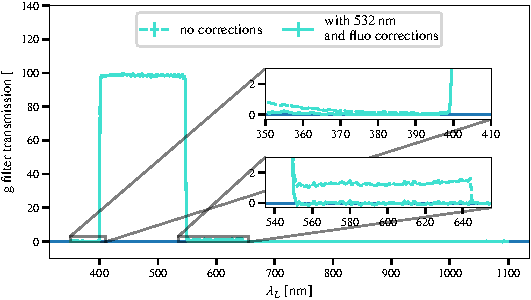
\includegraphics[width=\columnwidth]{fig/g_filter_532.pdf}
    \caption{\SD g filter transmission as a function of the set laser wavelength $\lambda_L$, with and without the \SI{532}{\nm} and fluorescence correction. For clarity, we added a zoom on the out-of-band transmission where $\SI{532}{\nm}$ line is transmitted while higher wavelengths are shot by the laser.}
    \label{fig:g_filter_532}
    %cbp_paper_plots.ipynb
\end{figure}


\subsection{Pinhole intercalibration}

Because we use a different pinhole for the CBP response and the \SD response measurement, we must intercalibrate the CBP response with both pinholes. The CBP response $\Rcbp$ defined in Equation~\ref{eq:rsd} can be developed as follows:

\begin{equation}
	\Rcbp(\lambda) \equiv \Rcbp^{\spinhole}(\lambda) = \Rcbp^{\bpinhole}(\lambda) \times \Kpinholes,
\end{equation}
with $\Kpinholes$ the intercalibration term and $\Rcbp^{\spinhole}$ (resp. $\Rcbp^{\bpinhole}$) the CBP response measured with the \spinhole pinhole (resp. \bpinhole pinhole). 

We estimate the correction term $\Kpinholes$ as the ratio of the \SD responses obtained with both pinholes from runs No.~8. The \bpinhole pinhole photometry is performed as follows. The background is estimated with dark exposures from the dark datasets, and the spatial mean of all these dark images is computed to obtain a master dark. When performing aperture photometry on the \bpinhole image, we subtract a background equivalent to the aperture photometry of the master dark at a similar position and radius, obtaining $\Qccd^{\bpinhole}$. The optimal radius is evaluated at 300 pixels for the \bpinhole pinhole to contain the main spot and the 1\up{st} order ghost. Figure~\ref{fig:stardice_5mm_response} shows the \SD response obtained with the \bpinhole pinhole and no filter. 

%We could have increased the radius to contain the iris flux, but it would have added as much noise as the signal gained. 

\begin{figure}[h]
    \centering
    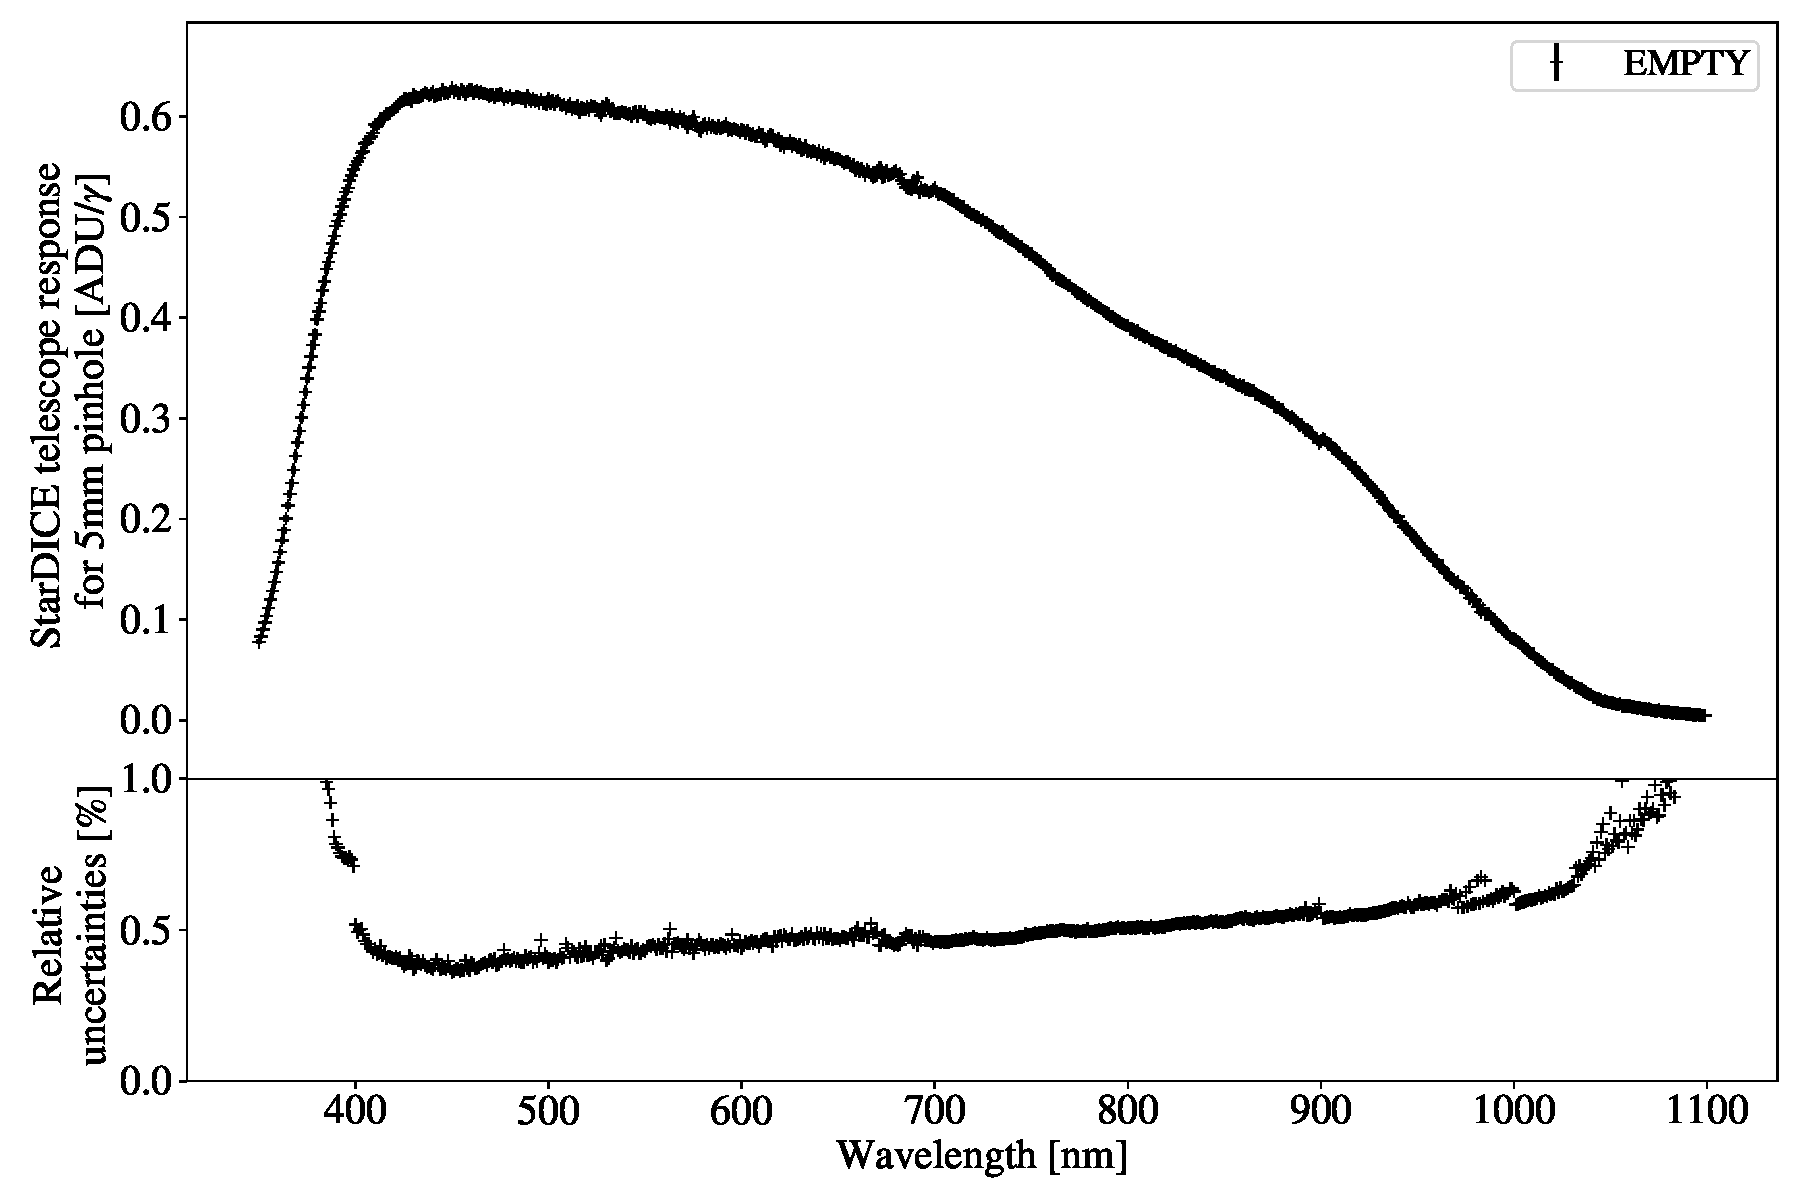
\includegraphics[width=\columnwidth]{fig/stardice_5mm_response.pdf}
    \caption{\textit{Top:} \SD response with no filter and \bpinhole pinhole with respect to wavelength in nanometer. \textit{Bottom:} Uncertainties over the \SD response measurement with respect to wavelength in nanometer.}
    \label{fig:stardice_5mm_response}
    %~/stardice/analysis/cbp_paper/golden_sample_analysis/dr2/response_plots.ipynb
\end{figure}

%When shooting with the \bpinhole pinhole, the main spot is not a pointlike source, hence the data reduction of $\Qccd^{\bpinhole}$ is different than the baseline photometry. The overscan subtraction and the light contamination correction are done with the same method as the \spinhole pinhole, detailed in \ref{sec:photometry_small}. However, the background subtraction cannot be performed the same way. 

%When using \bpinhole pinhole, the main spot takes a significant area of the focal plane, meaning there is not enough background in the image to reconstruct it. The background contribution is estimated by aperture photometry in the master dark at the same position and same radius as the laser-on images. $\Qccd^{\bpinhole}$ is measured with aperture photometry, after background subtraction. The optimal radius is evaluated at 300 pixels for the \bpinhole pinhole to contain the main spot and the 1\up{st} order ghost. We could have increased the radius to contain the iris flux, but it would have added as much noise as the signal gained. 

To compare the \SD responses for both pinholes, we need to measure the fluxes with aperture photometry at the same radius so that they contain the same features, such as the ghost contribution. This way there is no other consideration than the geometry of the pinholes. We estimate the \spinhole pinhole flux $F(300, \lambda)$. We compute the ratio $\Kpinholes=\frac{F(300)}{\Qccd^{\bpinhole}}$ and show the result in Figure~\ref{fig:ratio_pinholes}. The linear fit of this ratio is used to intercalibrate the \bpinhole pinhole $\Rcbp(\lambda)$ obtained and the \spinhole pinhole \SD for every measurement of this analysis.

%The non-null slope and not expected as the ratio between the two pinholes should correspond only to the ratio of surfaces of the illuminated area at the input CBP. We suspect that some light diffusion on the edges of the pinholes or other complex reflections in the setup could give this ratio a chromatic dependence.
\begin{figure}[h]
    \centering
    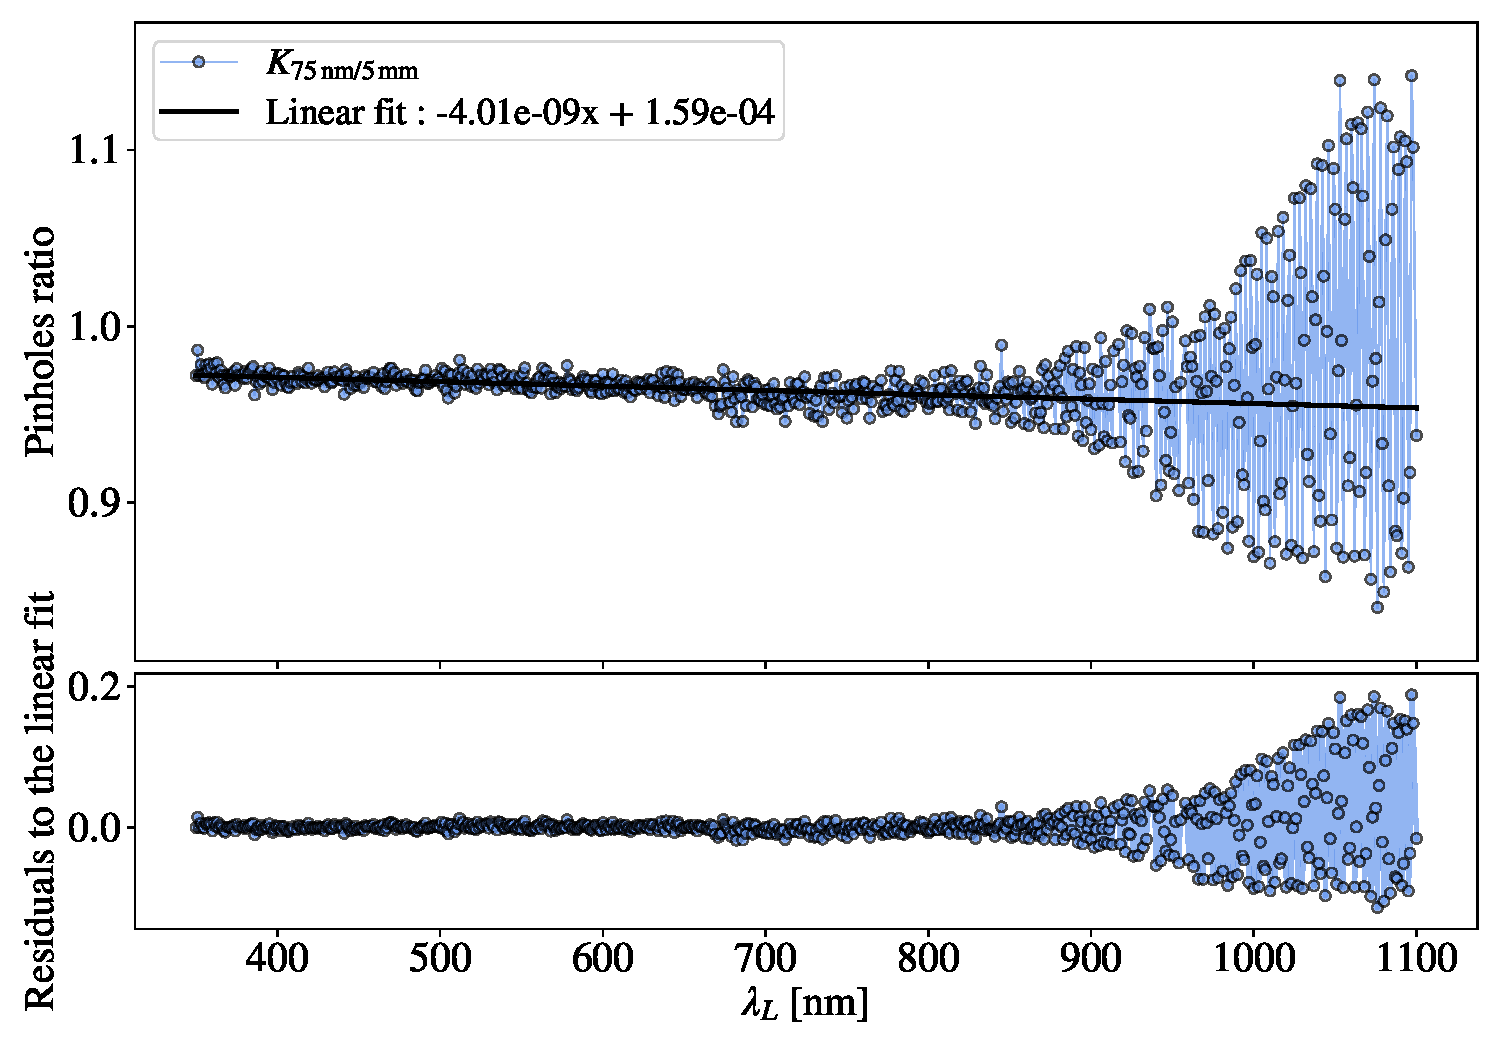
\includegraphics[width=\columnwidth]{fig/ratio_pinholes.pdf}
    \caption{Ratio $\Kpinholes$ as a function of wavelength, relative to the prediction given by the ratio of the nominal area of the pinholes. The black line corresponds to a linear fit between \SI{400}{\nm} and \SI{900}{\nm}.}
    \label{fig:ratio_pinholes}
    %~/stardice/analysis/cbp_paper/total_fluxes/ratio_pinholes.ipynb
\end{figure}


\subsection{Photometry applicable to on-sky data}
\label{sec:photometry_small}

The measurement of the PSF at a long distance from its core is possible in CBP images because of the very low level of background light in these images. It is impractical to port this method to on-sky data. We choose to carry out the throughput measurement for an aperture photometry and a background estimation algorithm applicable to on-sky data. 

The photometry is performed as follows. To estimate the background contribution, the sources in the image need to be detected and masked. We compute the standard deviation of an image $\sigma$, and every pixel with a signal higher than 5$\sigma$ is masked, as well as all the surrounding pixels that have a signal higher than 2$\sigma$. Then we proceed to a segmentation of the masked image into boxes of $129\times132$ pixels. We compute the mean and the standard deviation of the background in each of these boxes, and we interpolate their values in a 2D map to get our estimation of the background. This background estimation is subtracted from the image. Then, the centroid of the spot of interest is computed to pursue aperture photometry at this position. $\Qccd$ is measured with aperture photometry at a radius of \SI{20.9}{pixels} for every image of the dataset with the \spinhole.

Based on the model built in Sect.~\ref{sec:modelisation-sd-psf}, we can quantify the fraction of the total flux measured in \spinhole pinhole images with this aperture photometry method. We define the fraction of flux missed as the ratio between the value measured with aperture photometry for a given radius and wavelength and the total amplitude $A$ fitted with the method detailed in the previous section for the same wavelength. The result is given as the blue curve in Figure~\ref{fig:bias_aperture}. About 98\% of the flux is collected between \SI{400}{\nano\meter} and \SI{900}{\nano\meter}. The ghost contribution, which is missed when using an aperture of \SI{20.9}{pixels}, contributes about another extra percent to the missed flux below \SI{400}{\nano\meter}. Above \SI{900}{\nano\meter} where the PSF is degrading fast, the fraction of flux missed increases by one order of magnitude and reaches more than 75\% at \SI{1050}{nm}.

While most of this effect is directly explained by the aperture correction, a small contribution also comes from a bias in the background estimate, caused by the pollution of the background map by the source PSF tails. Given that the model of the PSF predicts the value of the aperture correction (red curve in Fig.~\ref{fig:bias_aperture}), we can estimate the contribution of the background bias as the difference between the two curves. This curve, presented in the bottom panel of Fig.~\ref{fig:bias_aperture}, shows that the background bias contributes about 0.2\% of the total flux.

\begin{figure}[h]
     \centering
     \resizebox{\hsize}{!}{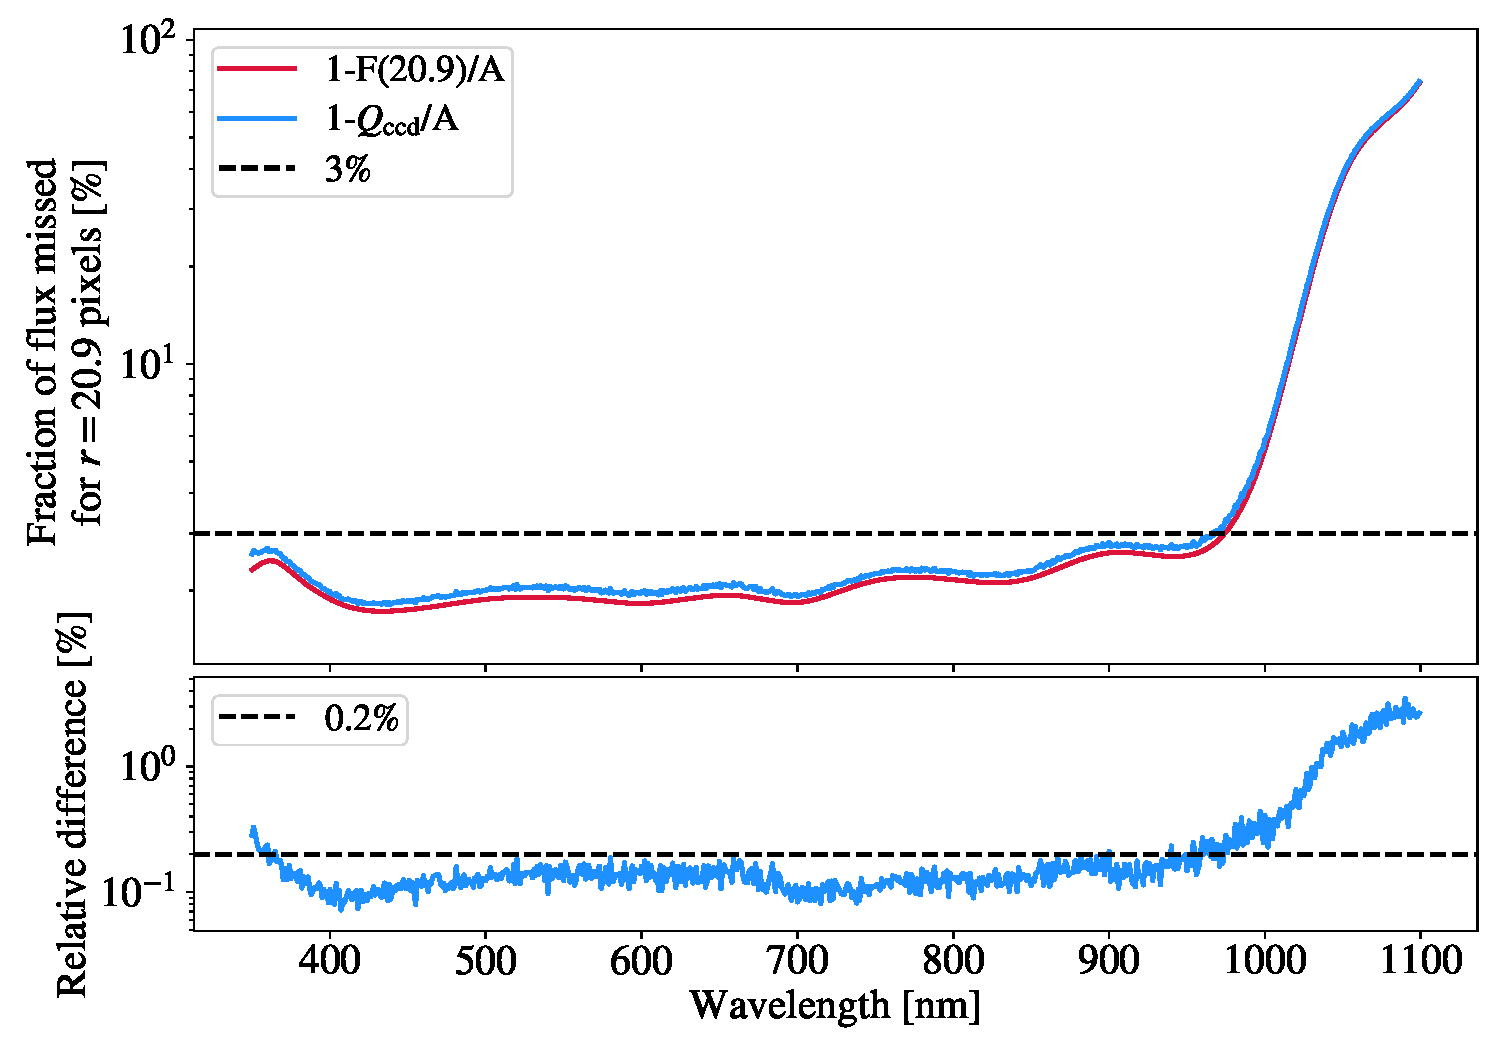
\includegraphics{fig/bias_aperture.pdf}}
     \caption{\textit{Top:} Fraction of missing flux against $\lambda_L$ when measuring \spinhole pinhole dataset with aperture photometry at \SI{20.9}{pixels} rather than taking the total amplitude $A$ fitted. The red curve corresponds to the estimation of the fit, the green one to aperture photometry when the background is estimated with the dark datasets, and the blue one to aperture photometry when the background is estimated with the method described in Section~\ref{sec:photometry_small}. \textit{Bottom:} Relative difference in percent between the flux measured for aperture photometry with the two background estimations and the model estimation at \SI{20.9}{pixels}.}
     \label{fig:bias_aperture}
    %~/stardice/analysis/cbp_paper/total_fluxes/fit_results.ipynb
\end{figure}

%
% TODO une conclusion qui dit: Les résultats sont valables pour cette photométrie, si la PSF sur le ciel n'est pas trop différente. Entre 900 et 400 ça devrait faire gros. Mais au-delà va savoir. Les résultats seront révisés quand on aura la PSF sur le ciel
% 
We conclude that the instrument response determined for our large aperture photometry of the \spinhole pinhole is likely to be applicable to similar star photometry with minimal aperture corrections in the range between \SI{400}{\nano\meter} and \SI{900}{\nano\meter}. Below \SI{400}{\nano\meter} there will be a need to take into account the ghosting pattern for the full aperture which will mix partially with the photometry aperture. Above \SI{900}{\nano\meter}, our method is unlikely to give a representative determination of the response of the instrument to star flux. At this stage we think that the \SD telescope is responsible for the PSF degradation, with one possible explanation being that the primary mirror becomes partially transparent and generates diffused light. Further discussion of the applicability of the measured transmission to on sky data will require study of the PSF on stellar images and is left for future work.


% The bottom panel corresponds to the aperture correction that is needed to apply to the aperture photometry measurement. It is around 2\% below \SI{950}{\nano\meter}, and increases by one order of magnitude in the infrared. This increase is correlated with the variation of the Moffat parameters $\alpha$ and $\beta$, showing that the PSF is drastically changing in the near-infrared. This issue is discussed in more details section \ref{sec:ir}. The third panel shows a constant background against wavelength, at a mean of \SI{0.27}{ADU/pixel}.
%
%\subsubsection{Summary}
%
%The summary of the error budget on the \SD telescope response id detailed in Figure~\ref{fig:sd_budget}
%
%
%\begin{figure}
%    \centering
%    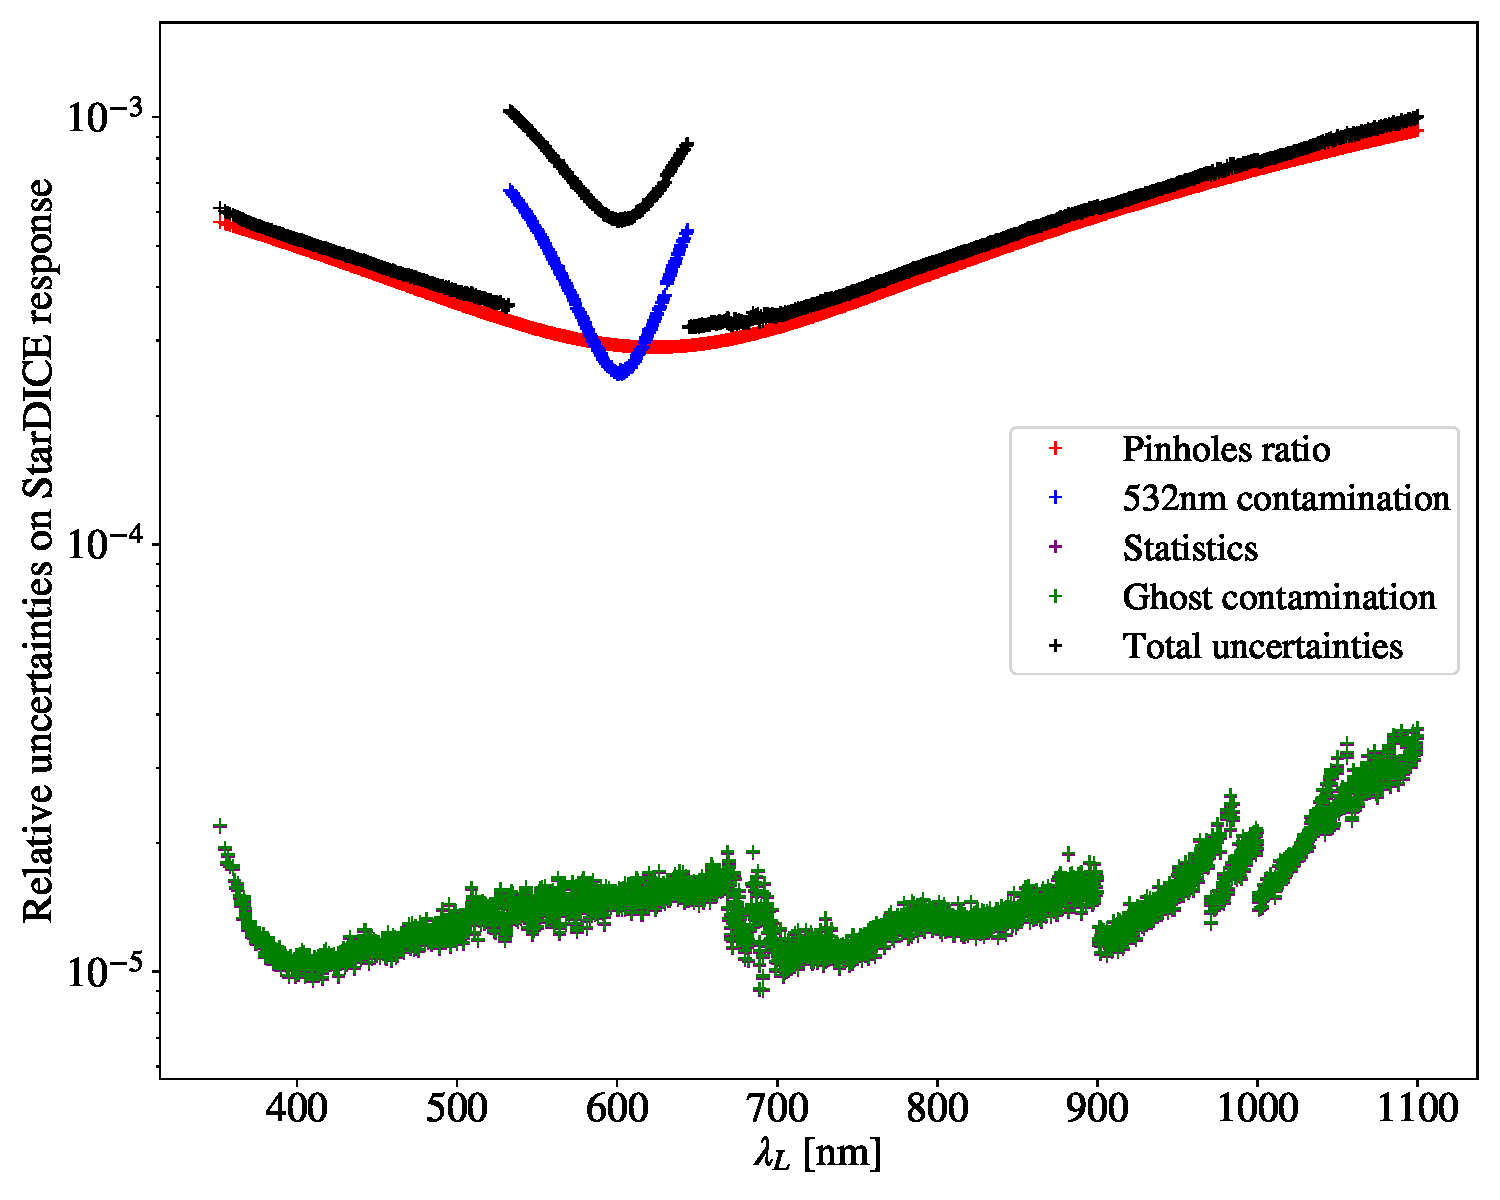
\includegraphics[width=\columnwidth]{fig/sd_uncertainties_budget.pdf}
%    \caption{Total error budget for \SD response.}
%    \label{fig:sd_budget}
%\end{figure}

\subsection{Results}
\subsubsection{\SD response and filter transmissions}

We measured the \SD response with the empty slot of the filterwheel, and the transmission of the $ugrizy$ filters, as well as the grating transmission with dataset No.~6, using the \spinhole pinhole, shooting at a fix mirror and focal plane position. Figure~\ref{fig:stardice_75um_response} shows the results obtained, following the procedure based on aperture photometry. We note that the wavelength coverage does not scan the full passband of the $u$ filter. Filling the gap between our measurements and the atmospheric UV cut off would need additional measurements out of the scope of this paper.

After accounting for the relative uncertainties, we demonstrate a precision of \textasciitilde\SI{0.5}{\%} for all the filter transmissions, the empty filterwheel slot, and the 1$^\mathrm{st}$ order of the diffraction grating from \SIrange{400}{950}{\nano\meter}. The \SI{0.2}{nm} wavelength accuracy of our measurements is illustrated by the fine resolution of the sharp filter edges.



\begin{figure}[h]
    \centering
    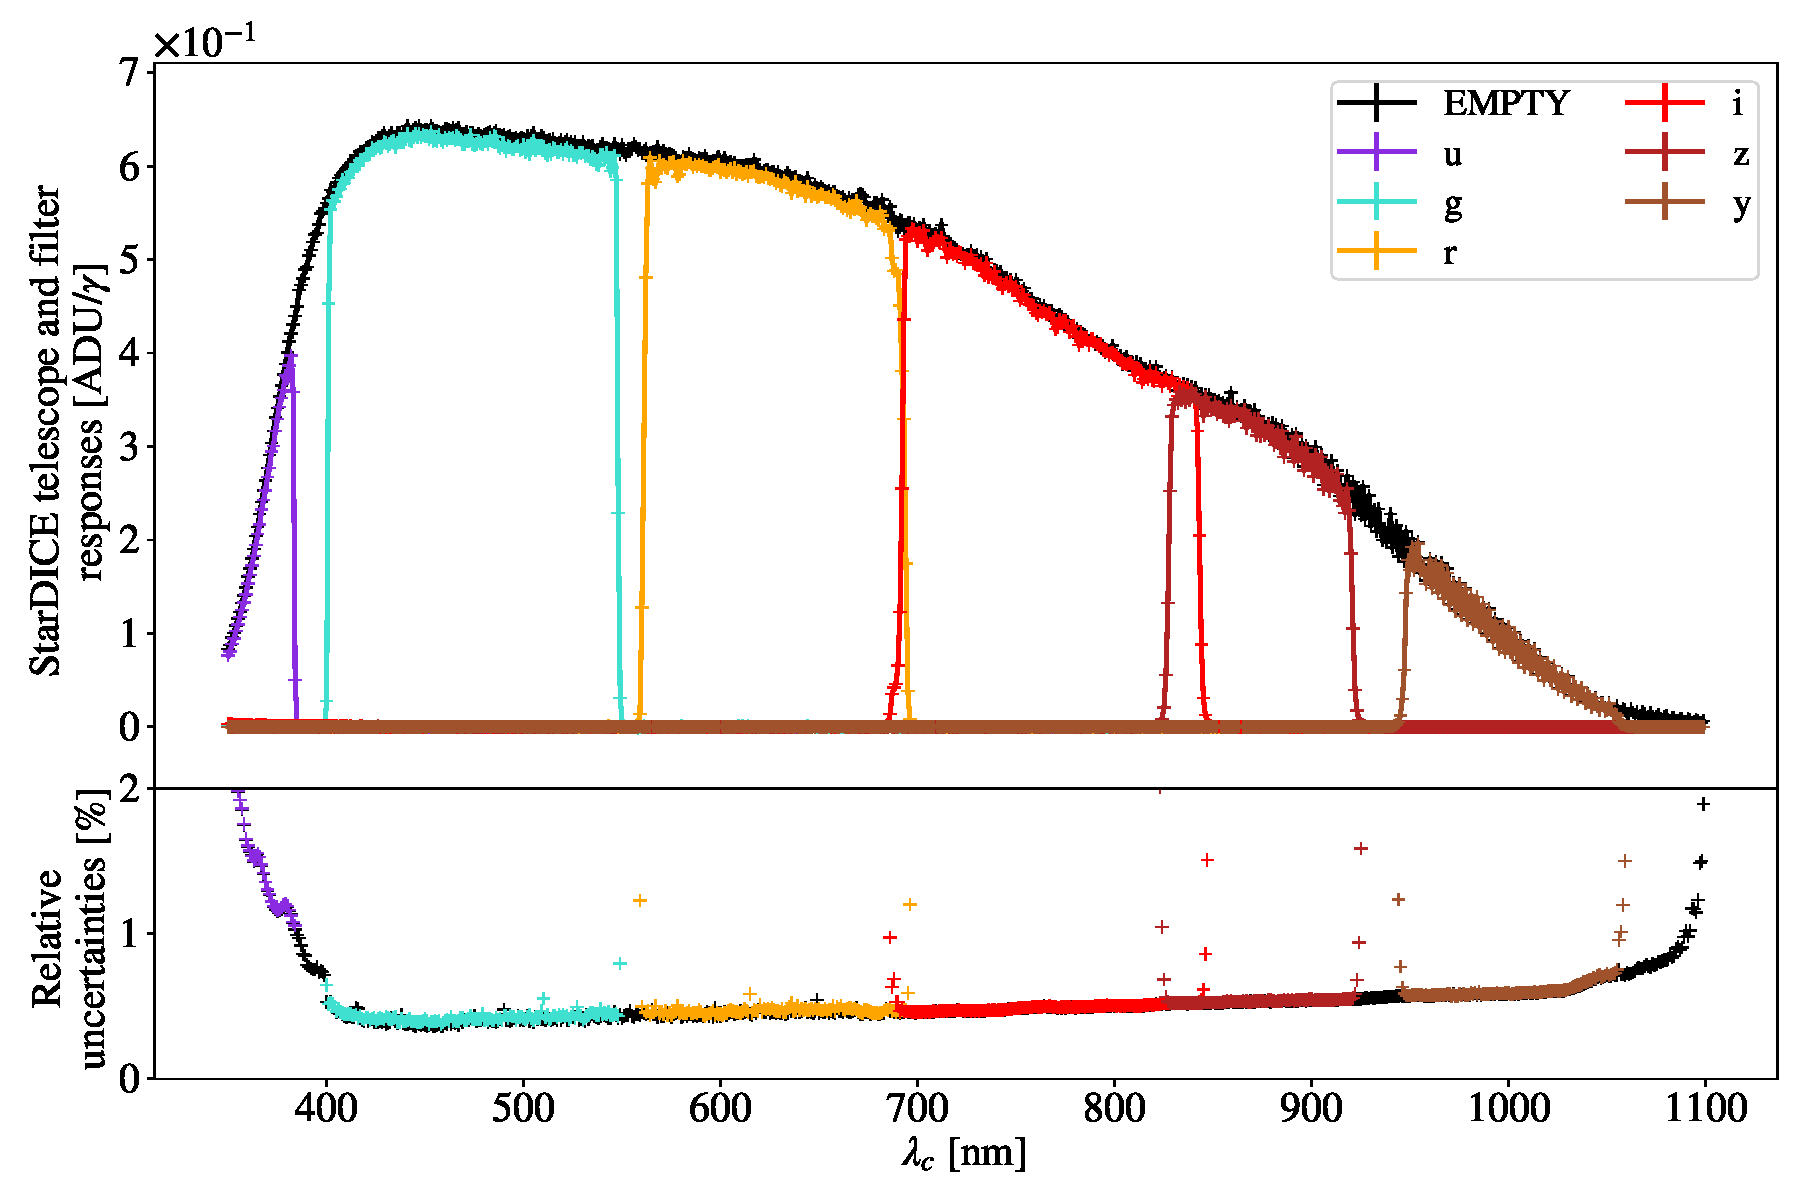
\includegraphics[width=\columnwidth]{fig/stardice_75um_response.pdf}
    \caption{\textit{Top}: \SD response against wavelength in nanometer, with the empty filterwheel slot; all $ugrizy$ filters; and the 0$^\mathrm{th}$, 1$^\mathrm{st}$ and 2$^\mathrm{nd}$ order diffraction of the grating. All of these responses have been measured with the \spinhole pinhole. \textit{Bottom:} Relative uncertainties over the \SD response measurements against wavelength in nanometer.}
    \label{fig:stardice_75um_response}
    %~/stardice/analysis/cbp_paper/golden_sample_analysis/dr5/response_plots.ipynb
\end{figure}

%\begin{figure}[h]
%    \centering
%    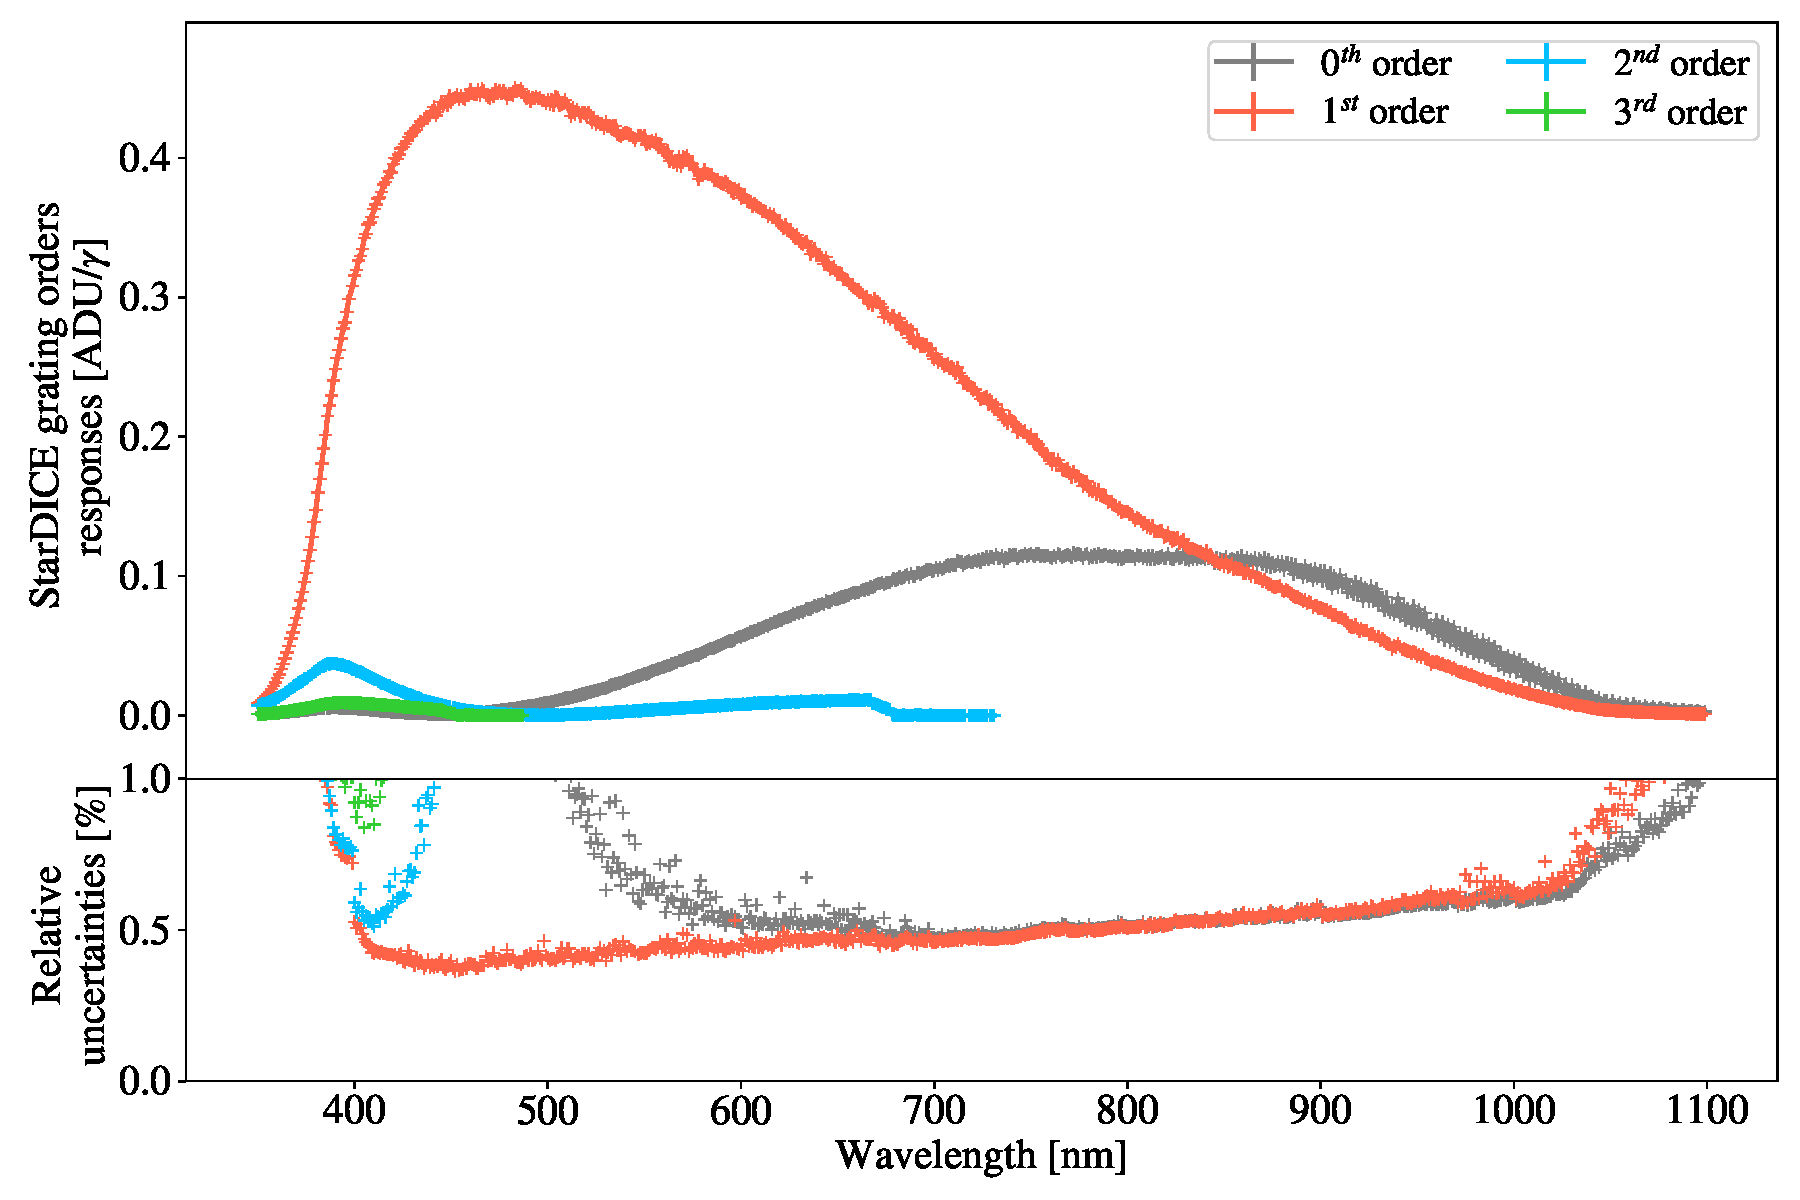
\includegraphics[width=\columnwidth]{fig/stardice_grating_response.pdf}
%    \caption{\textit{Top:} \SD response with the grating in front of the camera and \spinhole pinhole with respect to wavelength in nanometer. \textit{Bottom:} Uncertainties over the \SD response measurement with respect to wavelength in nanometer.}
%    \label{fig:stardice_grating_response}
%    %~/stardice/analysis/cbp_paper/golden_sample_analysis/dr2/response_plots.ipynb
%\end{figure}

\subsubsection{\SD Responses variations}

Since the CBP only illuminates a portion of the primary mirror, we need several measurements at different positions in order to span the full behavior of the \SD telescope. Dataset No.~2, where we point at 4 different positions along the primary mirror radius, and No.~3 were we point at every one of the four quadrants of the primary mirror, have been acquired specifically to investigate these variations. We also explored the small scale variations over the focal plane with Dataset No.~12, where we make slight pointing changes around a fixed positions.


%This paper focuses on dataset No.2, as it is used to synthesize the full pupil transmission in Section\ref{sec:pupil_stitching}. The \SD responses for the four radial mirror positions (see Figure\ref{fig:8_mirror_positions}) are shown in the left panel of Figure \ref{fig:radial_positions}.
Figure \ref {fig:radial_positions} displays the results of the transmission measurements in different quadrants (Dataset No.~3) on its left panel, and the variations over the focal plane (Dataset No.~12) on its right panel.

For both datasets, we display the average behavior by fitting a smooth spline through the different measurements. The variations in the red, above \SI{900}{\nano\meter} are due to small scale variations caused by interference fringing in the detector. As expected, their impact is larger when the optical path differences between measurements is smaller, i.e. when we explore the variations over the focal plane (right panel).

The most striking feature of figure \ref{fig:radial_positions} needing discussion is the large (\SI{20}{\%}) variation of transmission measured in the different quadrants of the primary mirror below \SI{400}{\nano\meter}. We didn't reach a firm conclusion concerning the explanation of this behavior, but the more solid assumption is that it might be explained by the Hilux coating\footnote{\url{https://www.orionoptics.co.uk/optical-coatings/}} on the \SD mirrors, whose reflectivity varies with the light incidence angle

In the 400-\SI{900}{\nano\meter} region, the variations over the focal plane and
between primary mirror quadrants are below the percent level. This relative
homogeneity of the telescope response allows to pursue the modeling of the full
pupil response of the instrument expecting a reasonable accuracy without the
need of additional data, as discussed further in section
\ref{sec:pupil_stitching}.

Also regarding the modeling of the full pupil transmission,
figure~\ref{fig:blueshift} shows the measurement of the expected interference
filter edges shift caused by the incident light angle variation when we
illuminate the primary mirror at different radii. The figure shows the edges of
the $g$ and $r$ filter in the top panel, and of the $z$ and $y$ filters in the
bottom panel as measured when illuminating four different radial positions in
Dataset No~2. The edges are noticeably bluer at higher radial positions, which
correspond to higher incidence angles, illustrating how the accuracy of those
measurements allows to consider their interpolation in order to obtain the full
pupil transmission of the telescope.


\textbf{Il faut une légende qui donne la position angulaire pour la figure 43}


\begin{figure*}[ht]
    \centering
    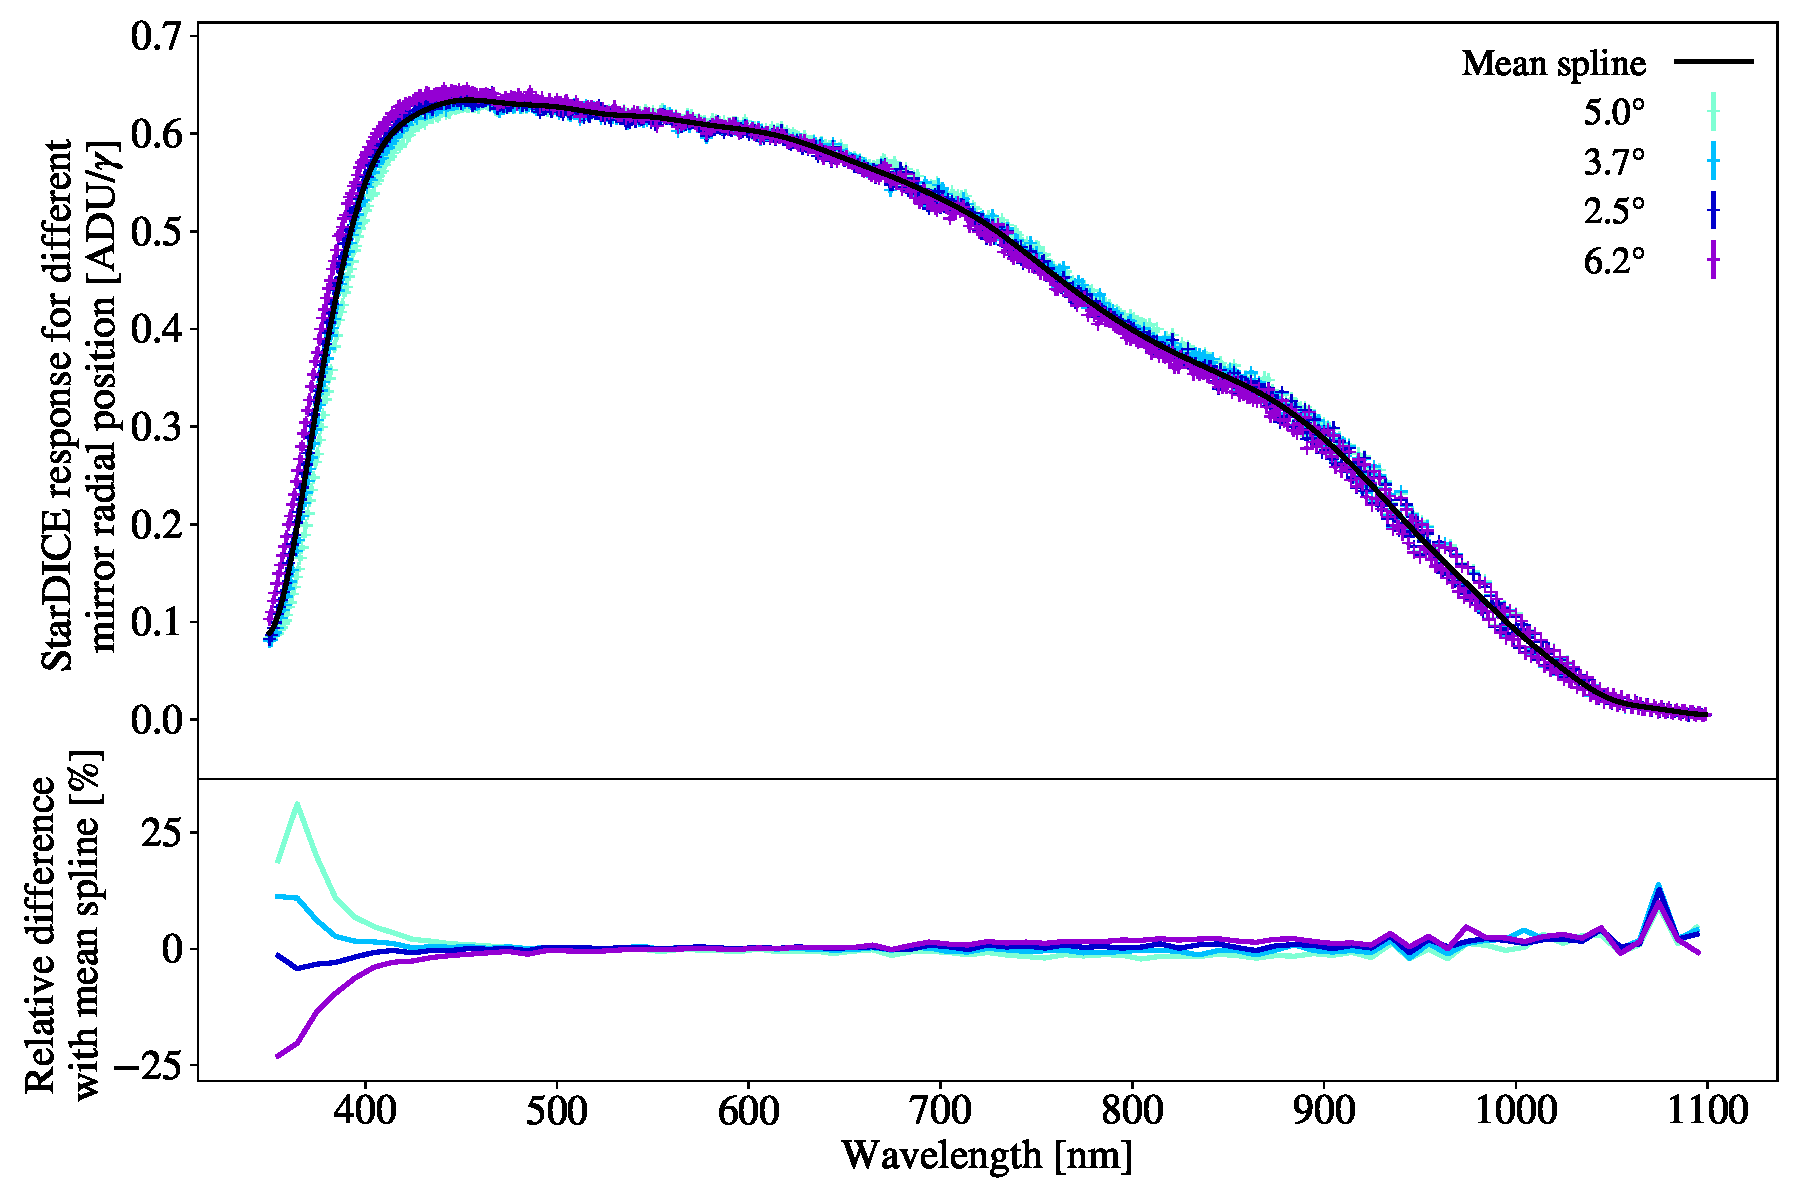
\includegraphics[width=\columnwidth]{fig/radial_positions.pdf}
    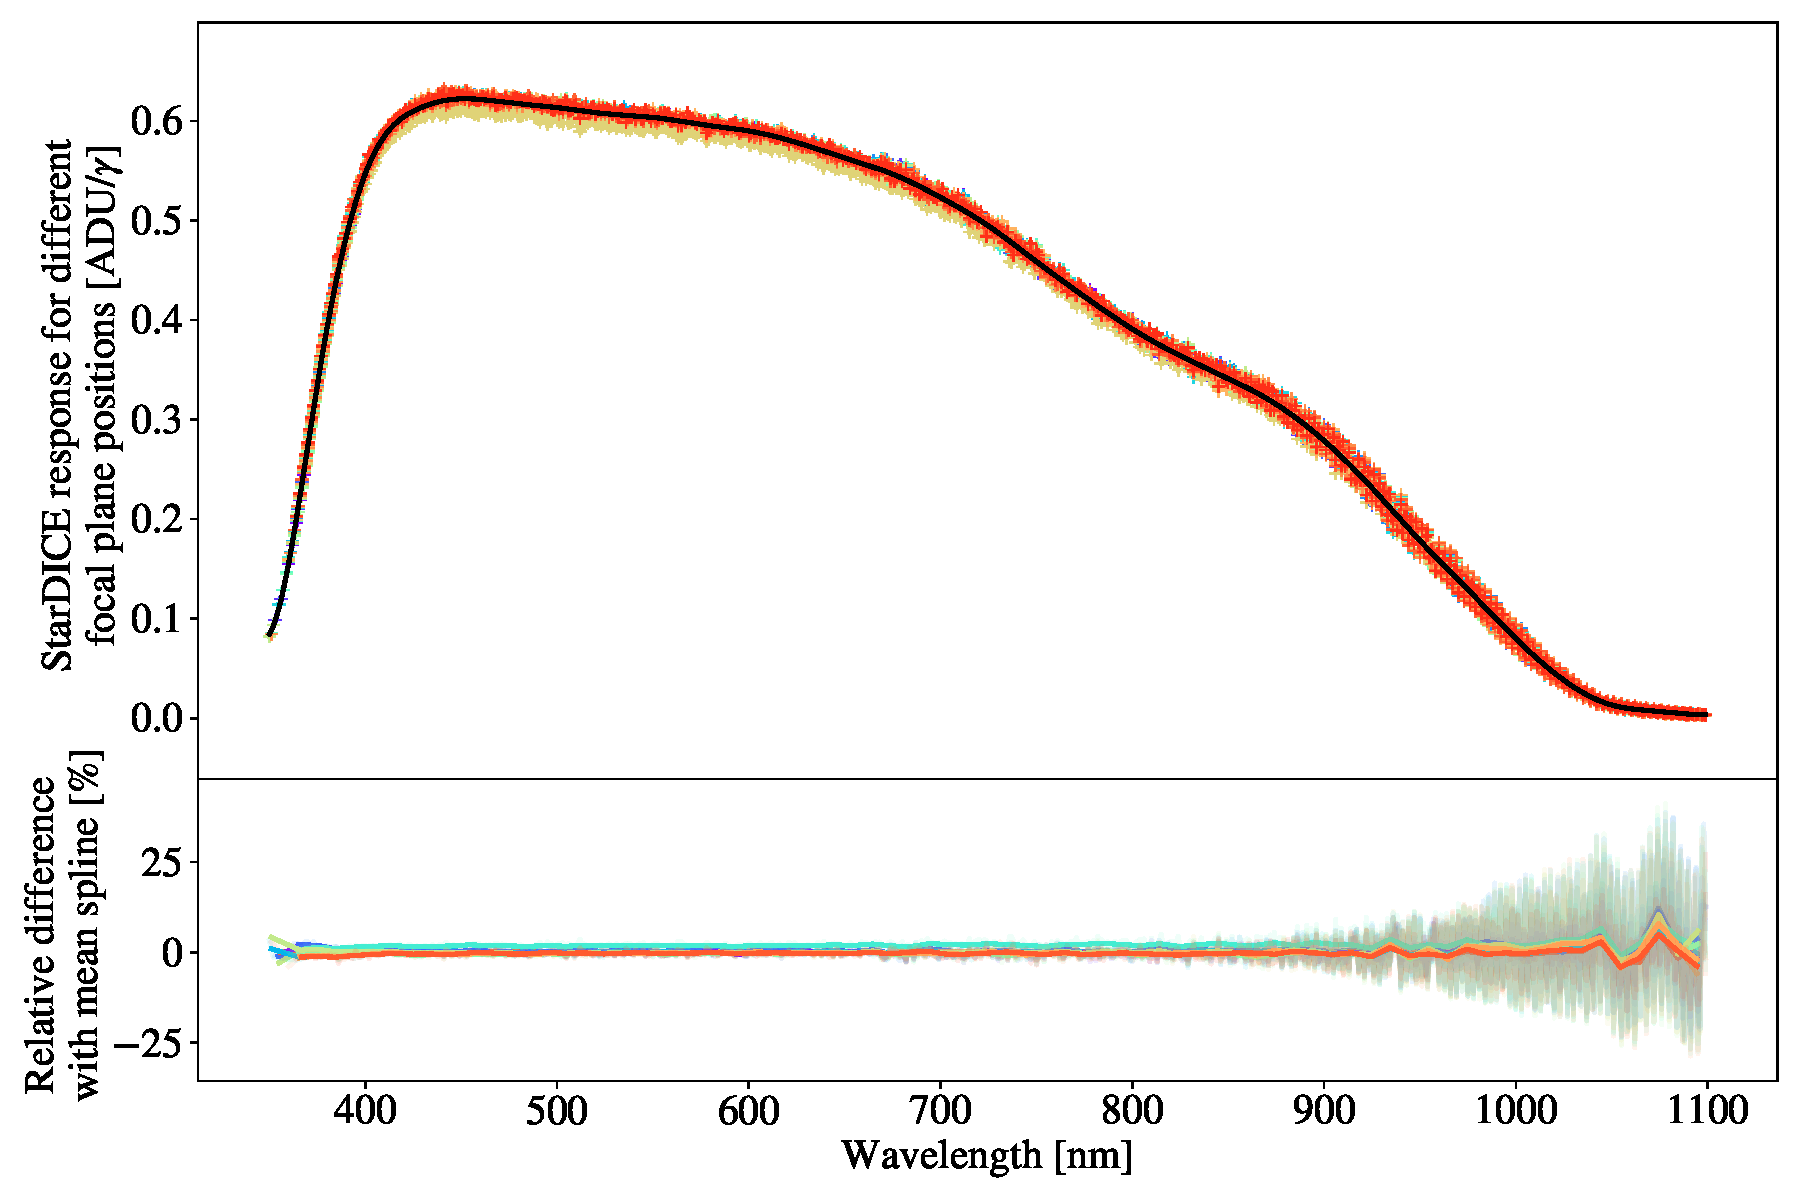
\includegraphics[width=\columnwidth]{fig/ccd_positions.pdf}
    \caption{\textit{Top:} \SD response for the different radial positions on the mirror with a fix focal plane position (left), and different focal plane positions  with a fix mirror position (right). The colors are matching with positions illustrated in Figures~\ref{fig:8_mirror_positions} and \ref{fig:ccd_grid}, and the black dashed line correspond to the mean spline. \textit{Bottom:} Relative difference between the data and the mean spline, binned to a \SI{10}{\nano\meter} resolution.}
    \label{fig:radial_positions}
    %~/stardice/analysis/cbp_paper/golden_sample_analysis/dr5/2022_03_01_stardice_transmission_radius.ipynb
\end{figure*}

\begin{figure}
    \centering
    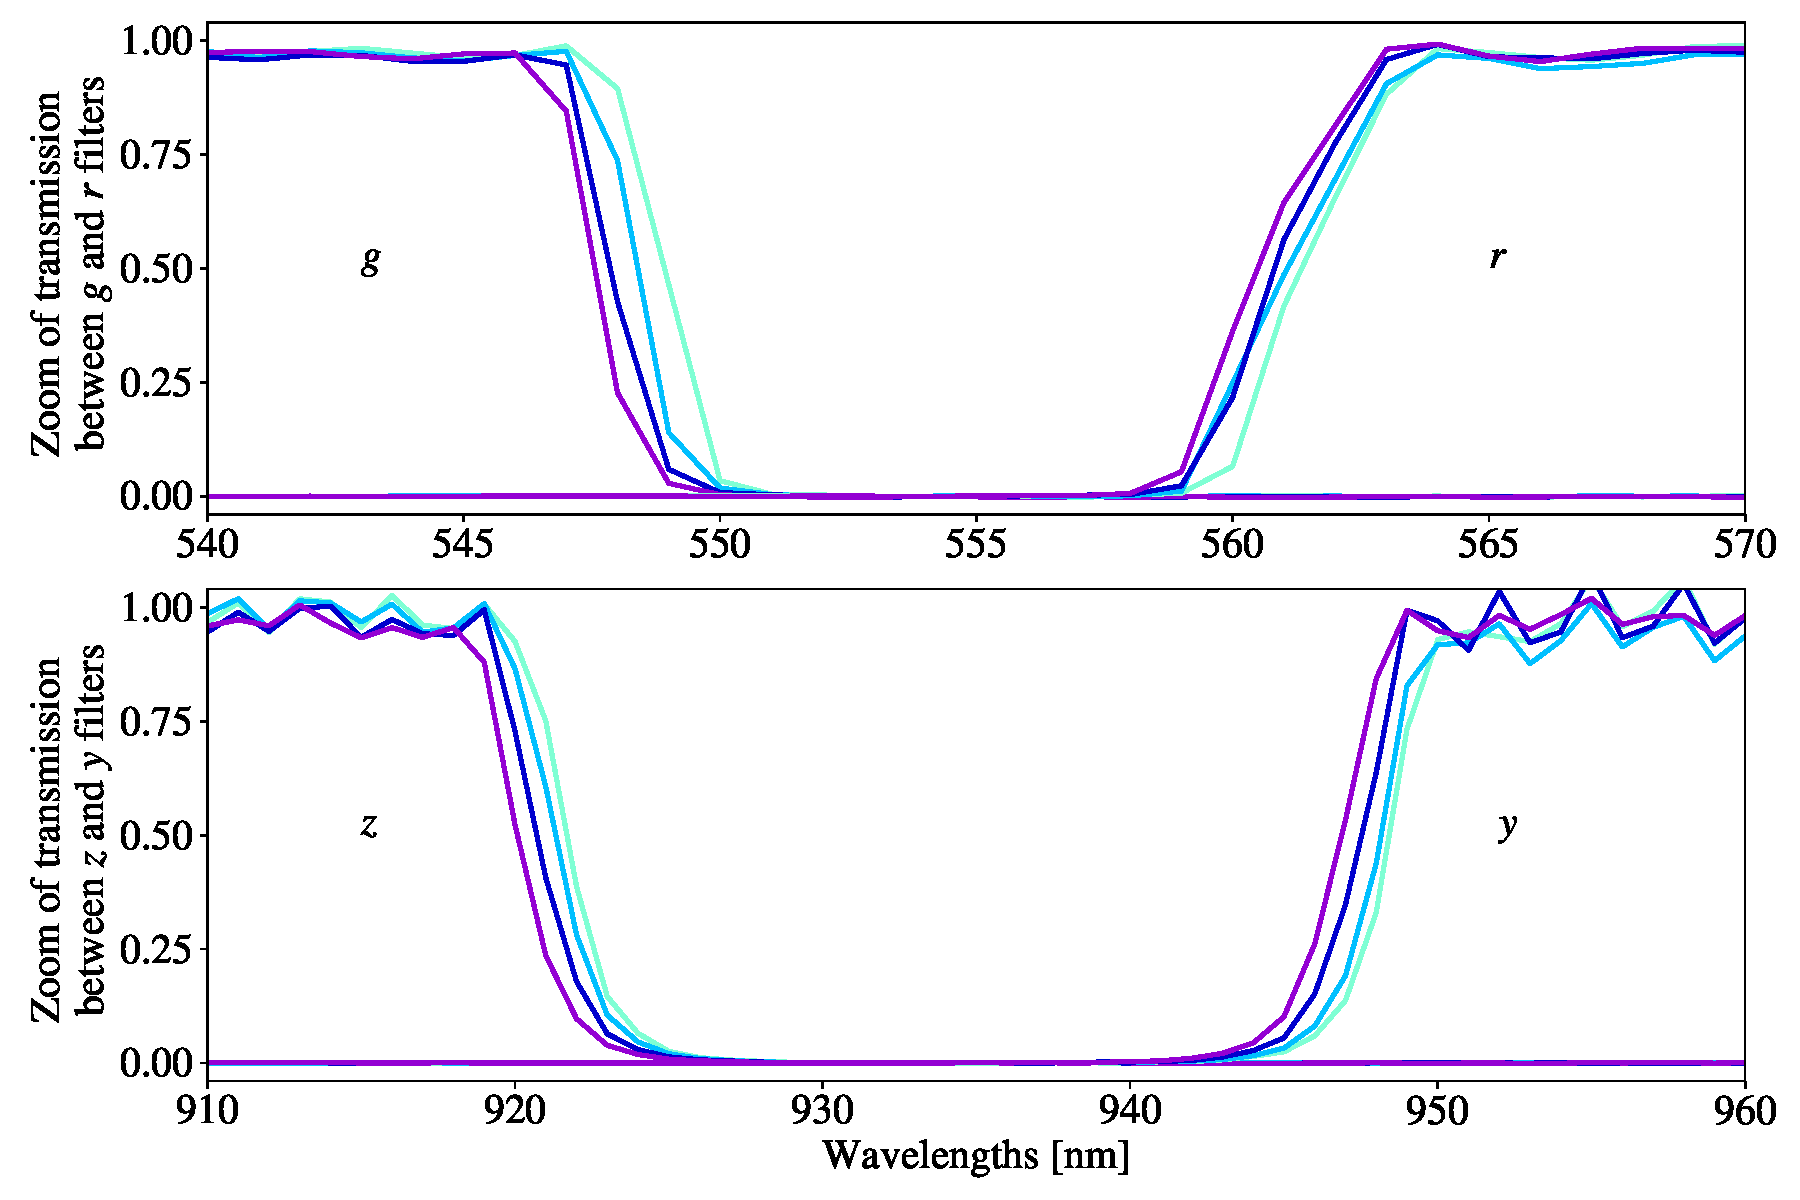
\includegraphics[width=1\columnwidth]{fig/blue_shift_filter_edges.pdf}
    \caption{Zoom on the \SD filter transmissions measured at different radial positions on the mirror, between the $g$ and $r$ filters (top panel) and the $z$ and $y$ filters (bottom panel). The colors are matching with positions illustrated in Figure~\ref{fig:8_mirror_positions}.}
    \label{fig:blueshift}
\end{figure}

%\subsubsection{Quadrant positions}
%
%The upper Figure~\ref{fig:radial_positions} shows the \SD response obtained with the \spinhole pinhole and without filters for the different quadrant positions on the mirror shown in Figure~\ref{fig:8_mirror_positions} right, and the same focal plane position. The lower figure shows the normalized residuals to the mean spline going through the four responses. We see again a divergence below \SI{400}{\nm} of about 20\% at most. The phenomenon in the infrared is still caused by the fringing. 
%
%\begin{figure}[h]
%    \centering
%    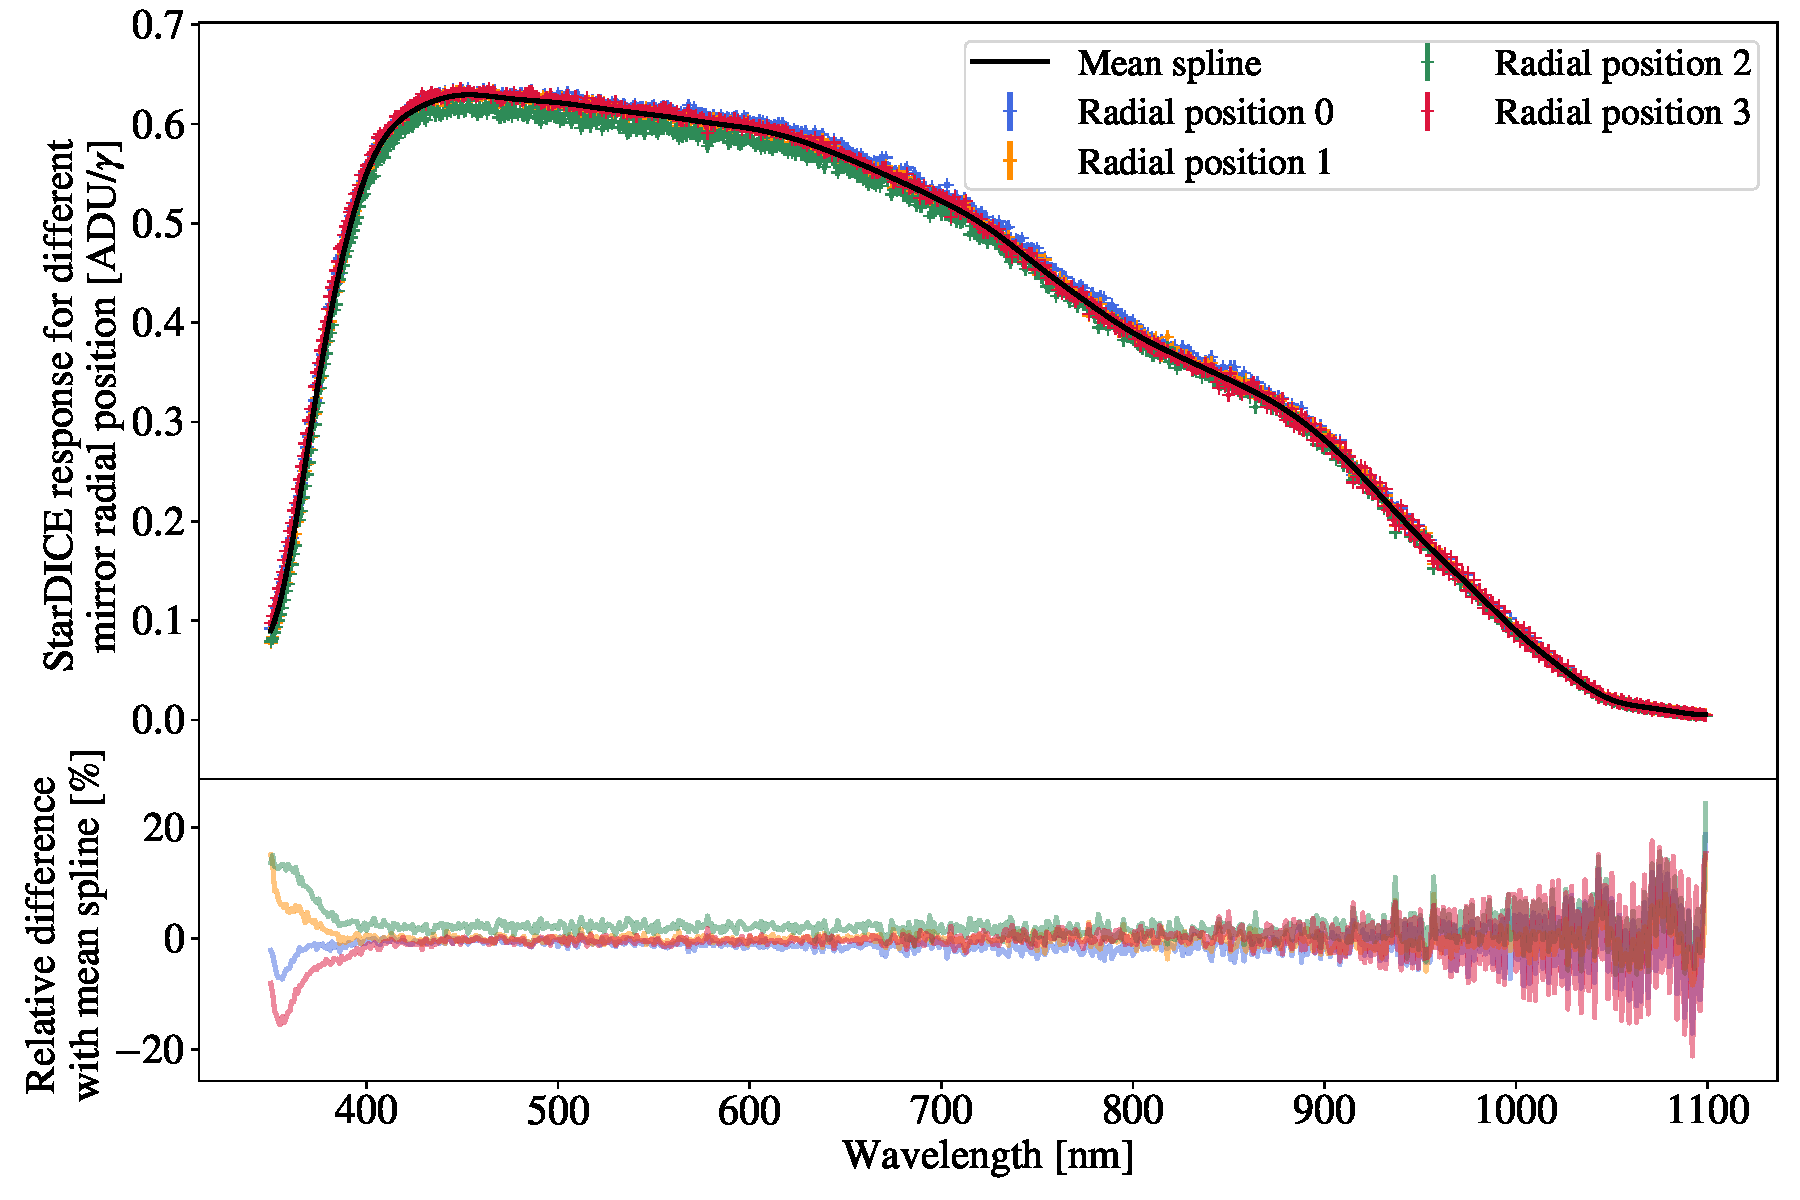
\includegraphics[width=\columnwidth]{fig/quadrant_positions.pdf}
%    \caption{\textit{Top:} \SD response for the different quadrant positions on the mirror, but the same position on the focal plane. \textit{Bottom:} Relative difference between the data and the mean spline.}
%    \label{fig:quadrant_positions}
%    %~/stardice/analysis/cbp_paper/golden_sample_analysis/dr2/2022_03_01_stardice_transmission_mirror_samples.ipynb
%\end{figure}









